% Perception par marqueurs ArUco -- Rock Climbing Robots
% Compilation : latexmk -xelatex perception_aruco.tex   (XeLaTeX : polices du Mac)
\documentclass[11pt,a4paper]{article}

\usepackage[a4paper,margin=2.3cm,headheight=14pt]{geometry}
\usepackage{fontspec}
\setmainfont{Charter}
\setsansfont{Avenir Next}
\setmonofont{Menlo}[Scale=0.84]
\usepackage[french]{babel}
\usepackage{amsmath,amssymb}
\usepackage{graphicx}
\usepackage{booktabs,array,tabularx}
\usepackage{xcolor}
\usepackage{listings}
\usepackage{enumitem}
\usepackage{caption,subcaption}
\usepackage{float}
\usepackage{fancyhdr}
\usepackage{titlesec}
\usepackage{microtype}
\usepackage{tikz}
\usetikzlibrary{arrows.meta,positioning,calc,fit,backgrounds,shapes.geometric,babel,decorations.pathreplacing}
\usepackage[most]{tcolorbox}
\usepackage[hidelinks]{hyperref}

% ---- couleurs ------------------------------------------------------------------------------------------
\definecolor{accent}{HTML}{1F5FA8}
\definecolor{wallc}{HTML}{E2C99A}
\definecolor{codebg}{HTML}{F4F6F8}
\definecolor{okgreen}{HTML}{2E8B57}
\definecolor{axx}{HTML}{D62728}
\definecolor{axy}{HTML}{2CA02C}
\definecolor{axz}{HTML}{1F77B4}
\definecolor{holdc}{HTML}{C2185B}

% ---- mise en page ----------------------------------------------------------------------------------------
\titleformat*{\section}{\Large\bfseries\sffamily\color{accent}}
\titleformat*{\subsection}{\large\bfseries\sffamily}
\titleformat*{\subsubsection}{\normalsize\bfseries\sffamily}
\pagestyle{fancy}
\fancyhf{}
\fancyhead[L]{\small\sffamily Rock Climbing Robots --- Perception ArUco}
\fancyhead[R]{\small\sffamily\thepage}
\renewcommand{\headrulewidth}{0.4pt}
\setlength{\parskip}{0.45em}
\setlength{\parindent}{0pt}
\captionsetup{font=small,labelfont={bf,sf}}
\setlist{itemsep=0.15em,topsep=0.3em}

% ---- code ------------------------------------------------------------------------------------------------
\newcommand{\code}[1]{\texttt{\detokenize{#1}}}
\lstdefinestyle{base}{basicstyle=\ttfamily\small, backgroundcolor=\color{codebg}, frame=single,
  rulecolor=\color{gray!40}, framesep=4pt, xleftmargin=6pt, xrightmargin=6pt, columns=fullflexible,
  keepspaces=true, showstringspaces=false, breaklines=true, aboveskip=0.6em, belowskip=0.6em,
  commentstyle=\color{gray}, keywordstyle=\color{accent}\bfseries, stringstyle=\color{okgreen}}
\lstdefinestyle{py}{style=base, language=Python}
\lstdefinestyle{sh}{style=base, language=bash, keywordstyle=\color{black}}
\lstdefinestyle{out}{style=base, backgroundcolor=\color{black!85}, basicstyle=\ttfamily\scriptsize\color{white},
  rulecolor=\color{black}}
\lstset{style=base}

% ---- encadrés ----------------------------------------------------------------------------------------------
\newtcolorbox{retenir}[1][À retenir]{colback=accent!5, colframe=accent, fonttitle=\bfseries\sffamily,
  title=#1, arc=2pt, boxrule=0.8pt, breakable}
\newtcolorbox{attention}[1][Attention]{colback=orange!6, colframe=orange!80!black, fonttitle=\bfseries\sffamily,
  title=#1, arc=2pt, boxrule=0.8pt, breakable}

% ---- styles TikZ -------------------------------------------------------------------------------------------
\tikzset{
  box/.style={draw=#1!70!black, fill=#1!10, rounded corners=2pt, align=center, font=\small,
              minimum height=10mm, text width=36mm, inner sep=3pt},
  box/.default=gray,
  arr/.style={-{Stealth[length=2.4mm]}, thick, gray!60!black},
  ax/.style={-{Stealth[length=2mm]}, very thick},
}

\begin{document}

% =========================================================================================================
\begin{titlepage}
\centering
\vspace*{2.5cm}
{\sffamily\color{accent}\Huge\bfseries Perception par marqueurs ArUco\par}
\vspace{0.6cm}
{\sffamily\Large Hackathon Rock Climbing Robots --- règlement v1.1, section 6.1\par}
\vspace{1.2cm}
{\large Où sont les caméras ? Où est le robot ? Où sont les prises ?\\[0.2em]
Ce qui a été fait, comment ça marche, comment s'en servir\par}
\vspace{1.5cm}
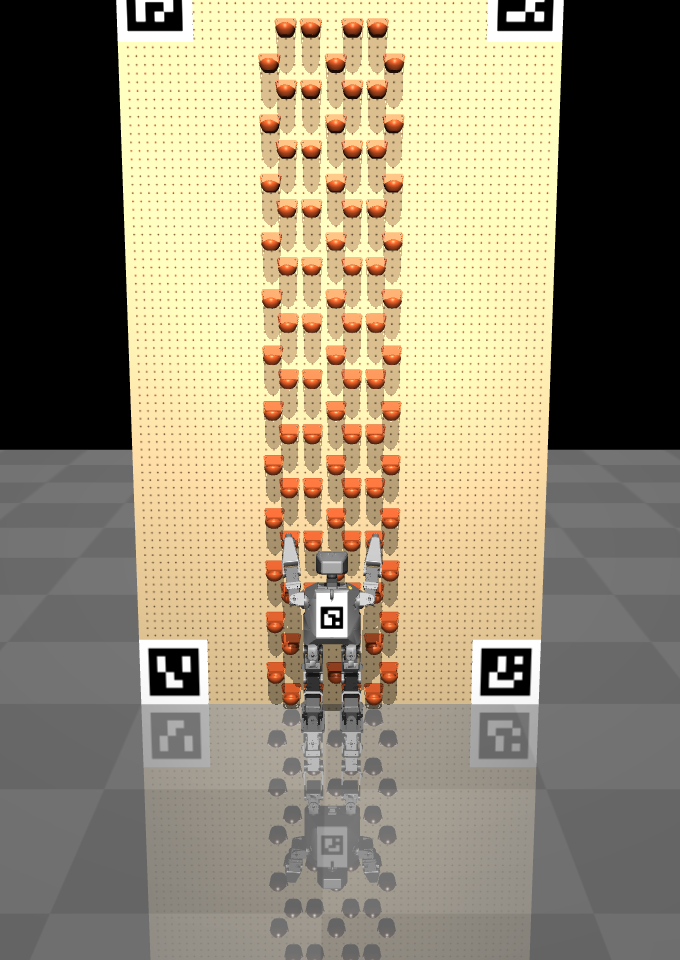
\includegraphics[width=0.36\textwidth]{img/scene.png}\hspace{0.04\textwidth}%
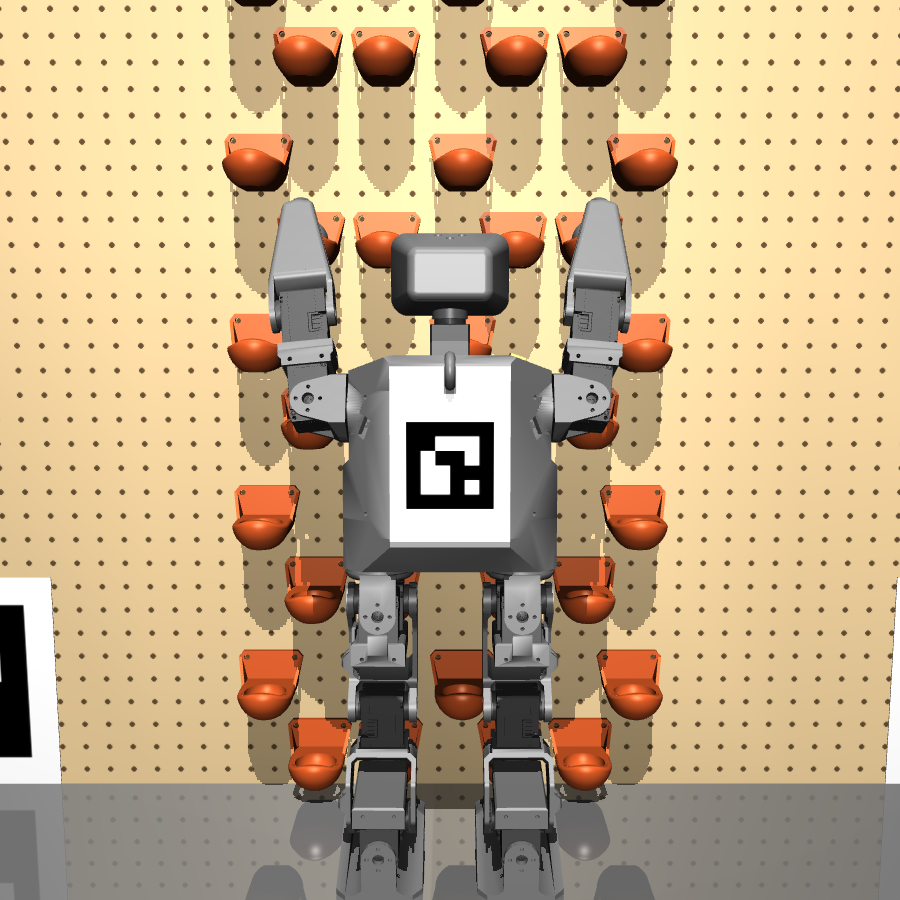
\includegraphics[width=0.36\textwidth]{img/robot_back.png}
\vfill
{\sffamily 29 octobre 2026\par}
\vspace{0.3cm}
{\small\color{gray} Document de travail de l'équipe. Code dans \code{Hackathon/perception/}.\par}
\end{titlepage}

\tableofcontents
\newpage

% =========================================================================================================
\section{En bref}

Le règlement (section 6.1) propose un mode de perception \emph{avec marqueurs ArUco} : quatre marqueurs
fixés aux coins du mur donnent la position des caméras, et un cinquième marqueur, collé sur le robot, donne
la position du robot. C'est ce mode qui a été programmé et testé dans le simulateur MuJoCo des
organisateurs, avec en plus la détection des prises.

\begin{retenir}[Ce qui marche aujourd'hui]
\begin{enumerate}
  \item \textbf{Les caméras se repèrent seules} : dans chaque image, le code trouve les marqueurs ID~1 à 4
        des coins du mur et en déduit où est la caméra et où elle regarde, \emph{sans qu'on le lui dise}.
        Précision : environ \textbf{2~mm} sur sa position, \textbf{0,02°} sur son orientation.
  \item \textbf{Le robot porte le marqueur ID~5 officiel} : l'autocollant de la fiche des organisateurs
        (code de 42~mm, à plat sur le dos), reproduit dans le simulateur.
  \item \textbf{Le robot est localisé} en croisant les deux caméras (en 1920~×~1080) et en prenant son
        inclinaison dans sa centrale inertielle (IMU) : erreur moyenne de \textbf{0,9 à 1,6~mm} (pire cas
        4,3~mm), sur les murs N1, N2, N3 et pour des caméras placées au hasard.
  \item \textbf{Les prises sont trouvées} par leur couleur, calées sur la grille de trous :
        \textbf{100~\%} des prises sur le mur vide, aucune fausse ; les prises cachées par le robot apparaissent
        dès qu'il bouge. Sur une \textbf{photo du vrai mur} : les \textbf{52 prises}, avec leur couleur.
  \item \textbf{Le même code servira sur le vrai robot} : un script (\code{live.py}) lit les caméras USB,
        se calibre sur les marqueurs du mur, trouve les prises et suit le robot en direct.
\end{enumerate}
\end{retenir}

\paragraph{Ce qui n'est pas encore fait.} Le robot ne grimpe pas encore : la démonstration le fait seulement
se balancer sur ses prises de départ. Il reste à écrire le programme de grimpe, à relier l'IMU du vrai robot à
\code{live.py}, et à tout essayer avec les vraies caméras (section~\ref{sec:suite}).

\paragraph{Les commandes à connaître} (à lancer depuis le dossier \code{Hackathon/simulator}) :

\begin{lstlisting}[style=sh]
# 1. demonstration dans le simulateur, avec une fenetre (mur N1, N2 ou N3)
uv run --with opencv-contrib-python python ../perception/demo.py N2 --show
# 2. la video de la demonstration
open ../perception/out/demo.mp4
# 3. la meme chose avec les cameras placees au hasard (le nombre change le placement)
uv run --with opencv-contrib-python python ../perception/demo.py N2 --shuffle 3
# 4. le jour J : les deux cameras USB (gauche puis droite)
uv run --with opencv-contrib-python python ../perception/live.py 0 1
\end{lstlisting}

% =========================================================================================================
\section{Le contexte}

\subsection{Ce que dit le règlement}

\begin{itemize}
  \item \textbf{Section 5.1} --- deux caméras USB par mur (Intel RealSense D435i), une de chaque côté,
        \emph{fournies et placées par les organisateurs}. Les équipes branchent les câbles sur leur
        ordinateur et récupèrent les images. \textbf{Seule l'image couleur (RGB) est autorisée} (pas la
        profondeur).
  \item \textbf{Section 5.2} --- quatre marqueurs aux coins du mur, IDs 1 à 4, dictionnaire
        \code{DICT_4X4_50}. Chacun : code noir de 100~×~100~mm entouré d'une bordure blanche de 18~mm
        (plaque de 136~×~136~mm), le coin extérieur de la plaque sur le coin du mur. L'équipe peut ajouter un
        marqueur \textbf{ID~5 sur son robot} ; les organisateurs en fournissent une fiche à imprimer
        (section~\ref{sec:marqueur}).
  \item \textbf{Section 6.1} --- avec les marqueurs, les marqueurs du mur donnent la pose (position +
        orientation) des caméras par rapport au mur ; le robot est suivi grâce à son marqueur ID~5 (ou
        détecté autrement).
  \item \textbf{Section 8} --- utiliser les marqueurs multiplie le temps par \textbf{1,25} (le mode sans
        marqueur, plus difficile, garde ×1). La hauteur atteinte compte avant le temps : un robot fiable
        avec marqueurs bat un robot sans marqueur qui tombe.
\end{itemize}

\subsection{Le simulateur}

Le simulateur des organisateurs (\code{rock-climbing-robots/simulator}, paquet Python \code{climbing_sim})
contient le robot Microban et ses 19 moteurs, le mur de 800~×~1400~mm avec ses prises, les quatre
marqueurs des coins et deux caméras simulées qui ont les caractéristiques des D435i. Il ne contient pas de
marqueur sur le robot : on l'ajoute nous-mêmes (section~\ref{sec:marqueur}).

\begin{figure}[H]
\centering
\begin{tikzpicture}[x={(4.4cm,0cm)}, y={(0cm,3.6cm)}, z={(-0.5cm,-1.9cm)}, line join=round, font=\small]
  % mur
  \fill[wallc] (0,0,0) -- (0.8,0,0) -- (0.8,1.4,0) -- (0,1.4,0) -- cycle;
  \draw[thick, brown!60!black] (0,0,0) -- (0.8,0,0) -- (0.8,1.4,0) -- (0,1.4,0) -- cycle;
  % prises du mur N1
  \foreach \r in {2,7,...,87}{\foreach \c in {18,21,26,29}{
      \fill[orange!85!red] ({0.0325+\c*0.015},{-0.004+\r*0.015},0) circle (0.55pt);}}
  % marqueurs des coins
  \foreach \x/\y/\id in {0/1.264/1, 0.664/1.264/2, 0/0/3, 0.664/0/4}{
    \fill[white, draw=gray] (\x,\y,0) -- ++(0.136,0,0) -- ++(0,0.136,0) -- ++(-0.136,0,0) -- cycle;
    \fill[black] ({\x+0.018},{\y+0.018},0) -- ++(0.1,0,0) -- ++(0,0.1,0) -- ++(-0.1,0,0) -- cycle;
    \node[white, font=\scriptsize\bfseries\sffamily] at ({\x+0.068},{\y+0.068},0) {\id};}
  % robot (schématique) et son autocollant
  \draw[gray!60!black, line width=1.6pt] (0.3475,0.026,0.03) -- (0.36,0.17,0.12) (0.4225,0.026,0.03) -- (0.41,0.17,0.12);
  \draw[gray!60!black, line width=1.6pt] (0.3025,0.33,0.03) -- (0.34,0.27,0.12) (0.4675,0.33,0.03) -- (0.43,0.27,0.12);
  \fill[gray!55, draw=gray!40!black] (0.335,0.17,0.12) -- (0.435,0.17,0.12) -- (0.435,0.29,0.12) -- (0.335,0.29,0.12) -- cycle;
  \fill[white, draw=gray] (0.356,0.19,0.148) -- (0.414,0.19,0.148) -- (0.414,0.274,0.148) -- (0.356,0.274,0.148) -- cycle;
  \fill[black] (0.364,0.206,0.148) -- (0.406,0.206,0.148) -- (0.406,0.248,0.148) -- (0.364,0.248,0.148) -- cycle;
  % caméras et rayons
  \foreach \cx/\nm in {-0.15/gauche, 0.95/droite}{
    \foreach \tx/\ty in {0.068/1.332, 0.732/1.332, 0.068/0.068, 0.732/0.068}{
      \draw[orange!80!black, densely dashed, opacity=0.55] (\cx,0.9,2.4) -- (\tx,\ty,0);}
    \draw[okgreen, thick, opacity=0.85] (\cx,0.9,2.4) -- (0.385,0.227,0.148);
    \fill[black!80] (\cx,0.9,2.4) ++(-0.045,-0.03) rectangle ++(0.09,0.06);
    \node[below=1mm, align=center, font=\footnotesize] at (\cx,0.9,2.4) {caméra\\ \nm};}
  % repère du mur
  \draw[ax, axx] (0,0,0) -- (0.2,0,0) node[below right=-1mm, font=\footnotesize] {$x$};
  \draw[ax, axy] (0,0,0) -- (0,0.22,0) node[left, font=\footnotesize] {$y$};
  \draw[ax, axz] (0,0,0) -- (0,0,0.3) node[left, font=\footnotesize] {$z$};
  \node[anchor=east, align=right, font=\footnotesize] at (-0.07,0.55,0) {repère du mur\\origine : coin\\bas-gauche};
  % légende
  \node[anchor=west, align=left, font=\footnotesize] at (0.9,1.2,0)
     {\textcolor{orange!80!black}{- - -} vers les marqueurs 1--4\\[-1pt] \hspace{1.3em}(pose des caméras)\\[2pt]
      \textcolor{okgreen}{\rule[0.5ex]{1.4em}{1pt}} vers le marqueur 5\\[-1pt] \hspace{1.3em}(pose du robot)};
\end{tikzpicture}
\caption{Le dispositif (schéma, mur N1). Les deux caméras voient les quatre marqueurs des coins, ce qui
leur permet de se situer ; elles voient aussi le marqueur ID~5 sur le dos du robot, ce qui permet de situer
le robot, et les prises (en orange), qui sont repérées par leur couleur.}
\label{fig:dispositif}
\end{figure}

\subsection{Organisation des dossiers}

Tout est dans \code{~/Desktop/Hackathon} (dépôt GitHub \code{Alyaa203/Hackathon}). Les dépôts des
organisateurs (\code{simulator}) et de Rhoban (\code{microban}) n'y sont pas recopiés : ce sont des
\emph{sous-modules}, des liens vers la version exacte utilisée. Ils ne sont \textbf{pas modifiés} : notre code est
à part, dans \code{perception}.

\begin{lstlisting}
Hackathon/
|-- simulator/          depot des organisateurs (climbing_sim) -- sous-module, non modifie
|-- microban/           programme du vrai robot (Rhoban, branche dev_v2) -- sous-module
`-- perception/         NOTRE CODE
    |-- perception.py     le traitement : marqueurs, cameras, robot, prises
    |-- robot_marker.py   le marqueur ID 5 du robot (fiche des organisateurs) + simulateur
    |-- demo.py           demonstration dans le simulateur, comparee a la verite
    |-- live.py           le jour J : les vraies cameras USB (ou des images)
    |-- out/              produit par demo.py et live.py : demo.mp4, holds.json, images
    `-- doc/              ce document (perception_aruco.tex) et ses images
\end{lstlisting}

\begin{figure}[H]
\centering
\begin{tikzpicture}[node distance=9mm and 7mm]
  \node[box=accent] (demo) {\code{demo.py}\\\footnotesize démonstration (simulateur)};
  \node[box=accent, right=24mm of demo] (live) {\code{live.py}\\\footnotesize vraies caméras / images};
  \node[box=okgreen, below=of demo] (perc) {\code{perception.py}\\\footnotesize traitement d'image};
  \node[box=okgreen, below=of live] (mark) {\code{robot_marker.py}\\\footnotesize marqueur ID 5};
  \node[box=gray, below=of perc, xshift=-14mm] (cv) {OpenCV\\\footnotesize \code{cv2.aruco}, PnP};
  \node[box=gray, below=of mark, xshift=-12mm] (sim) {\code{climbing_sim}\\\footnotesize simulateur, dimensions};
  \node[box=gray, right=6mm of sim] (mj) {MuJoCo\\\footnotesize physique, rendu};
  \draw[arr] (demo) -- (perc);
  \draw[arr] (demo) -- (mark);
  \draw[arr] (live) -- (perc);
  \draw[arr] (live) -- node[right, font=\scriptsize, fill=white, inner sep=1pt]{constantes} (mark);
  \draw[arr] (perc) -- (cv);
  \draw[arr] (perc) -- node[pos=0.62, above, sloped, font=\scriptsize, fill=white, inner sep=1pt]{mur, prise} (sim);
  \draw[arr] (mark) -- (sim);
  \draw[arr] (mark) -- (mj);
  \draw[arr] (mark.south west) -- (cv);
\end{tikzpicture}
\caption{Qui utilise quoi. \code{perception.py} ne dépend que d'OpenCV et des dimensions du mur et de la prise
(données du simulateur) : il fonctionne aussi bien sur des images simulées que sur des images réelles.}
\end{figure}

\subsection{Installation}

Il faut \code{git}, \code{git-lfs} et \code{uv}. OpenCV n'est \emph{pas} ajouté au projet du simulateur (pour ne
pas modifier le dépôt des organisateurs) : on le demande à chaque lancement avec \code{--with}. \code{uv} le
télécharge la première fois (une minute) puis le garde en cache.

\begin{lstlisting}[style=sh]
git clone --recurse-submodules https://github.com/Alyaa203/Hackathon
cd Hackathon/simulator && uv sync
uv run --with opencv-contrib-python python ../perception/demo.py N1
\end{lstlisting}

\begin{attention}[Le message « VIRTUAL\_ENV ... does not match »]
Il apparaît quand un autre environnement Python (\code{tf_env}) est activé dans le terminal. Il est sans
conséquence (\code{uv} utilise bien l'environnement du simulateur). Pour le faire disparaître : \code{deactivate}.
\end{attention}

% =========================================================================================================
\section{Les repères}
\label{sec:reperes}

Toute la difficulté de la localisation est de passer d'un repère à l'autre. Il y en a cinq.

\begin{center}
\renewcommand{\arraystretch}{1.25}
\begin{tabularx}{\textwidth}{>{\bfseries}l X l}
\toprule
Repère & Axes & Utilisé par \\
\midrule
Mur $\mathcal{W}$ & origine au coin bas-gauche de la face avant ; $x$ à droite, $y$ vers le haut,
  $z$ sort du mur vers le grimpeur & marqueurs, caméras, résultats \\
Monde (MuJoCo) & même origine ; $x$ à droite, $y$ \emph{entre dans} le mur, $z$ vers le haut & simulateur, planification \\
Caméra $\mathcal{C}$ & convention OpenCV : $x$ à droite de l'image, $y$ vers le bas, $z$ devant la caméra & OpenCV \\
Marqueur $\mathcal{M}$ & centre du code ; $x$ à droite, $y$ vers le haut (vu de face), $z$ sort du marqueur & OpenCV \\
Tronc $\mathcal{T}$ & $x$ devant le robot (vers le mur quand il grimpe), $y$ à sa gauche, $z$ le long du dos & robot, IMU \\
\bottomrule
\end{tabularx}
\end{center}

Une \emph{pose} (position + orientation) d'un repère $\mathcal{B}$ dans un repère $\mathcal{A}$ s'écrit
avec une matrice de rotation $R_{AB}$ ($3\times3$) et une position $t_{AB}$ : un point de coordonnées
$P_B$ dans $\mathcal{B}$ a pour coordonnées dans $\mathcal{A}$
\[
  P_A = R_{AB}\,P_B + t_{AB}.
\]
Les \emph{colonnes} de $R_{AB}$ sont les axes de $\mathcal{B}$ exprimés dans $\mathcal{A}$. Pour passer du
mur au monde du simulateur, la rotation est fixe :
\[
  R_{\text{monde},\mathcal{W}} = \begin{pmatrix} 1 & 0 & 0\\ 0 & 0 & -1\\ 0 & 1 & 0\end{pmatrix}
  \qquad (x_{\text{monde}} = x,\quad y_{\text{monde}} = -z,\quad z_{\text{monde}} = y).
\]
C'est ce que fait la fonction \code{to_world()}.

% =========================================================================================================
\section{Les marqueurs ArUco}

\subsection{Qu'est-ce qu'un marqueur ArUco ?}

Un marqueur ArUco est un carré noir et blanc conçu pour être retrouvé facilement par un ordinateur. Pour le
dictionnaire \code{DICT_4X4_50} : une grille de $6\times6$ cases dont la couronne extérieure est noire et dont
les $4\times4$ cases intérieures codent un numéro (ID de 0 à 49). Autour, une bordure blanche le détache du
fond. Le motif n'est pas symétrique : en le lisant, OpenCV sait \emph{quel} marqueur il voit et \emph{dans
quel sens} il est tourné, donc il peut numéroter ses quatre coins toujours dans le même ordre.

\begin{figure}[H]
\centering
\begin{subfigure}[b]{0.46\textwidth}
\centering
\begin{tikzpicture}[scale=0.62, font=\footnotesize]
  \fill[white, draw=gray] (-0.75,-0.75) rectangle (6.75,6.75);
  \fill[black] (0,0) rectangle (6,6);
  \foreach \c/\r in {2/1,3/1,4/1, 1/2,4/2, 1/3,2/3, 1/4,2/4,4/4}{\fill[white] (\c,5-\r) rectangle ++(1,1);}
  \draw[gray!60, very thin] (0,0) grid (6,6);
  \foreach \p/\l/\a in {{(0,6)}/0/above left, {(6,6)}/1/above right, {(6,0)}/2/below right, {(0,0)}/3/below left}{
    \fill[red] \p circle (3.2pt); \node[\a=1pt, text=red, font=\small\bfseries] at \p {\l};}
  \draw[ax, axx] (3,3) -- (4.6,3) node[right, fill=white, inner sep=1pt] {$x$};
  \draw[ax, axy] (3,3) -- (3,4.6) node[above, fill=white, inner sep=1pt] {$y$};
  \fill[axz] (3,3) circle (4pt); \fill[white] (3,3) circle (1.6pt);
  \node[below right=-1pt, text=axz, fill=white, inner sep=1pt] at (3.1,2.9) {$z$};
  \draw[decorate, decoration={brace, amplitude=4pt, mirror}] (0,-1) -- (6,-1) node[midway, below=4pt] {code : 42 mm};
\end{tikzpicture}
\caption{Le marqueur ID~5 du robot. En rouge, l'ordre des coins rendu par OpenCV ; au centre, le repère du
marqueur ($z$ sort de la page).}
\end{subfigure}\hfill
\begin{subfigure}[b]{0.48\textwidth}
\centering
\begin{tikzpicture}[x=0.33mm, y=0.33mm, font=\footnotesize]
  \fill[wallc] (0,0) rectangle (190,175);
  \foreach \i in {0,...,11}{\foreach \j in {0,...,10}{\fill[brown!70!black] (17.5+\i*15,10+\j*15) circle (0.5);}}
  \fill[white, draw=gray] (0,0) rectangle (136,136);
  \fill[black] (18,18) rectangle (118,118);
  \fill[white] (43,43) rectangle (93,93);
  \node[font=\small\bfseries\sffamily, black] at (68,68) {3};
  \foreach \p/\l/\a in {{(18,118)}/0/above left, {(118,118)}/1/above right, {(118,18)}/2/below right, {(18,18)}/3/below left}{
    \fill[red] \p circle (2.2); \node[\a=0pt, text=red, font=\scriptsize\bfseries] at \p {\l};}
  \draw[thick, brown!50!black] (0,175) -- (0,0) -- (190,0);
  \draw[ax, axx] (0,0) -- (40,0) node[below] {$x$};
  \draw[ax, axy] (0,0) -- (0,40) node[left] {$y$};
  \draw[<->] (0,-12) -- (136,-12) node[midway, below] {136};
  \draw[<->] (0,-24) -- (18,-24) node[midway, below] {18};
  \draw[<->] (18,-24) -- (118,-24) node[midway, below] {100};
  \node[align=left, anchor=west, font=\scriptsize, fill=white, rounded corners=1pt, inner sep=2pt] at (140,60)
    {coins du code\\(mm, repère mur) :\\0 : (18, 118)\\1 : (118, 118)\\2 : (118, 18)\\3 : (18, 18)};
\end{tikzpicture}
\caption{Le marqueur ID~3 au coin bas-gauche du mur (motif simplifié). Ses coins ont des positions
\emph{connues} dans le repère du mur.}
\end{subfigure}
\caption{Anatomie d'un marqueur. Pour chaque coin, on connaît sa position en 3D (sur le mur, ou sur le
marqueur) et OpenCV donne sa position en pixels dans l'image : c'est cette double information qui permet
de tout localiser.}
\label{fig:aruco}
\end{figure}

\subsection{La détection : \texttt{detect()}}

OpenCV fait tout le travail : l'image est passée en niveaux de gris, les quadrilatères sombres sont repérés,
leur contenu est lu et comparé au dictionnaire. Deux réglages comptent :
\begin{itemize}
  \item l'\emph{affinage sous-pixel} des coins (\code{CORNER_REFINE_SUBPIX}) : la position des coins est précise
        à une fraction de pixel, ce qui compte beaucoup pour la précision finale ;
  \item la lecture de chaque case du code sur $8\times8$ pixels au lieu de $4\times4$
        (\code{perspectiveRemovePixelPerCell = 8}) : le code du robot ne fait qu'une vingtaine de pixels de côté
        dans les images, et avec le réglage par défaut OpenCV le trouvait mais n'arrivait pas à le lire sur
        environ une image sur six (25 images sur 31 lues pour une caméra) ; avec ce réglage, il le lit à chaque
        fois (31 sur 31).
\end{itemize}

\begin{lstlisting}[style=py]
_params = cv2.aruco.DetectorParameters()
_params.cornerRefinementMethod = cv2.aruco.CORNER_REFINE_SUBPIX
_params.perspectiveRemovePixelPerCell = 8
_detector = cv2.aruco.ArucoDetector(cv2.aruco.getPredefinedDictionary(cv2.aruco.DICT_4X4_50), _params)

def detect(image_rgb) -> dict[int, np.ndarray]:
    gray = cv2.cvtColor(np.ascontiguousarray(image_rgb), cv2.COLOR_RGB2GRAY)
    corners, ids, _ = _detector.detectMarkers(gray)
    if ids is None:
        return {}
    return {int(i): c.reshape(4, 2) for i, c in zip(ids.ravel(), corners)}
\end{lstlisting}

Le résultat est un dictionnaire \code{{ID: coins}}, chaque entrée contenant les 4 coins ($4\times2$ pixels)
dans l'ordre de la figure~\ref{fig:aruco}. Les positions 3D des coins des marqueurs du mur sont calculées par
\code{wall_marker_corners(id)} à partir des dimensions du règlement. La face avant des plaques est à
$z = 1$~mm du mur dans le simulateur (plaques de 1~mm d'épaisseur) : constante \code{PLATE_Z}.

% =========================================================================================================
\section{Étape 1 --- Où sont les caméras ?}
\label{sec:cameras}

\subsection{Le modèle de la caméra}

Une caméra (modèle « sténopé », celui d'OpenCV) transforme un point 3D en pixel en deux temps :

\begin{enumerate}
  \item \textbf{les extrinsèques} $(R, t)$ --- où est la caméra et où elle regarde --- font passer le point du
        repère du mur au repère de la caméra : $P_C = R\,P_W + t$ ;
  \item \textbf{les intrinsèques} $K$ --- propres à la caméra (focale $f_x, f_y$ et centre optique $c_x, c_y$
        en pixels) --- le projettent sur l'image :
\[
  \begin{pmatrix} u \\ v \\ 1 \end{pmatrix} \propto K\,P_C,
  \qquad
  K = \begin{pmatrix} f_x & 0 & c_x \\ 0 & f_y & c_y \\ 0 & 0 & 1 \end{pmatrix}.
\]
\end{enumerate}

Les intrinsèques se mesurent une fois pour toutes (calibration de la caméra, ou valeurs du fabricant). Les
extrinsèques changent dès qu'on bouge la caméra : ce sont elles qu'on cherche.

\subsection{Le problème PnP}

On connaît $n$ points 3D $P_i$ (les coins des marqueurs du mur) et leurs pixels $p_i$ dans l'image (donnés par
\code{detect()}). Trouver la pose $(R,t)$ de la caméra qui explique ces pixels s'appelle le problème
\textbf{PnP} (\emph{Perspective-n-Point}) :
\[
  (R, t) = \arg\min_{R,t} \sum_{i=1}^{n} \bigl\| \pi\bigl(K (R P_i + t)\bigr) - p_i \bigr\|^2
\]
où $\pi$ divise par la troisième coordonnée. Avec les 4 marqueurs, on a $n = 16$ coins, répartis aux quatre
coins du mur : c'est très contraint, donc très précis.

\begin{figure}[H]
\centering
\begin{tikzpicture}[font=\small]
  \fill[wallc] (4.2,-1.4) -- (7.6,-0.8) -- (7.6,2.8) -- (4.2,2.2) -- cycle;
  \node[font=\footnotesize, brown!50!black] at (6.9,2.35) {mur};
  \coordinate (C) at (0,0.6);
  \foreach \n/\P in {1/{(4.9,1.75)}, 2/{(7.1,2.1)}, 3/{(4.9,-0.7)}, 4/{(7.1,-0.3)}}{
    \coordinate (P\n) at \P;
    \fill[black] \P ++(-0.15,-0.15) rectangle ++(0.3,0.3);}
  \fill[gray!25, opacity=0.9, draw=gray] (1.5,-0.25) -- (1.9,-0.1) -- (1.9,1.45) -- (1.5,1.3) -- cycle;
  \node[font=\footnotesize, gray!40!black] at (1.7,1.75) {image};
  \foreach \n/\t in {1/0.336, 2/0.257, 3/0.336, 4/0.257}{
    \draw[orange!80!black, densely dashed] (C) -- (P\n);
    \fill[red] ($(C)!\t!(P\n)$) circle (1.6pt);}
  \fill[black] (C) circle (2pt) node[left] {$C$};
  \node[align=center, font=\footnotesize] at (0,-0.4) {centre optique\\ (inconnu)};
  \node[red, font=\footnotesize, align=center] at (2.2,-0.75) {$p_i$ : pixels\\détectés};
  \node[font=\footnotesize, align=center] at (6.0,0.7) {$P_i$ : coins des\\marqueurs, connus};
  \draw[ax, axz] (C) -- ++(0.9,0.12) node[above, font=\footnotesize] {$z_C$};
\end{tikzpicture}
\caption{Le problème PnP : on connaît les points du mur ($P_i$) et l'endroit où ils tombent dans l'image
($p_i$) ; on cherche la position et l'orientation de la caméra qui alignent chaque rayon.}
\end{figure}

\subsection{Le code : \texttt{camera\_pose()}}

\begin{lstlisting}[style=py]
def camera_pose(markers: dict, K, dist=None):
    ids = [i for i in WALL_IDS if i in markers]           # les marqueurs 1-4 vus
    if not ids:
        return None
    obj = np.concatenate([wall_marker_corners(i) for i in ids])  # points 3D (repere mur)
    img = np.concatenate([markers[i] for i in ids]).astype(np.float64)  # pixels
    ...
    _, rvec, tvec = cv2.solvePnP(obj, img, K, dist, flags=cv2.SOLVEPNP_IPPE)
    rvec, tvec = cv2.solvePnPRefineLM(obj, img, K, dist, rvec, tvec)
    proj, _ = cv2.projectPoints(obj, rvec, tvec, K, dist)
    rms = float(np.sqrt(np.mean(np.sum((proj.reshape(-1, 2) - img) ** 2, axis=1))))
    return rvec.ravel(), tvec.ravel(), rms
\end{lstlisting}

\begin{itemize}
  \item \code{SOLVEPNP_IPPE} est une méthode exacte pour des points tous dans un même plan (ici le mur) ; elle
        donne une première solution, que \code{solvePnPRefineLM} affine par moindres carrés.
  \item \code{rvec} est la rotation $R$ sous forme compacte (axe × angle, convertie par \code{cv2.Rodrigues}).
  \item \code{rms} est l'\textbf{erreur de reprojection} : on reprojette les 16 coins avec la pose trouvée et on
        mesure l'écart moyen avec les pixels détectés. Autour de 0,4~pixel : la pose explique très bien l'image.
        Plusieurs pixels : problème (mauvaises intrinsèques, marqueur mal détecté\ldots).
  \item La position de la caméra dans le repère du mur s'en déduit : $C = -R^\top t$.
\end{itemize}

\begin{retenir}
Le code n'a besoin de connaître \emph{que} les intrinsèques des caméras. Leur position est retrouvée à
chaque essai à partir des marqueurs du mur : les organisateurs peuvent placer les caméras où ils veulent,
tant que chacune voit les quatre coins. Il n'y a rien à mesurer au mètre.
\end{retenir}

% =========================================================================================================
\section{Étape 2 --- Le marqueur ID 5 sur le robot}
\label{sec:marqueur}

\subsection{La fiche des organisateurs}

Les organisateurs fournissent une fiche à imprimer, « \emph{ArUco marker ID 5 (DICT\_4X4\_50) for the robot's
back} ». Elle fixe tout : la taille du marqueur, sa place sur le robot et son repère.

\begin{center}
\renewcommand{\arraystretch}{1.2}
\begin{tabularx}{\textwidth}{l X}
\toprule
Élément & Valeur (fiche des organisateurs) \\
\midrule
Autocollant & 58,0~×~84,5~mm, avec en haut une encoche de 6,19~×~13,18~mm \\
Code noir & \textbf{42~mm} de côté \\
Où le coller & à plat sur le dos du robot (poitrine + capot) ; l'encoche glisse autour du pied de la poignée
               jusqu'en butée, ce qui le centre et le met à la bonne hauteur ; les côtés tombent sur les bords du dos,
               le bas sur la ligne entre la poitrine et le bassin \\
Centre du code & $(-33{,}0;\ 0;\ 54{,}75)$~mm dans le repère du tronc ($x$ devant, $y$ à gauche, $z$ en haut) \\
Axes du marqueur & $x = -y_T$ (vers la droite du robot), $y = +z_T$ (vers le haut), $z = -x_T$ (sort du dos) \\
Impression & à 100~\% (taille réelle, pas « ajuster à la page »), vérifier la règle de 100~mm, découper le contour \\
\bottomrule
\end{tabularx}
\end{center}

Le dos du tronc a été mesuré dans le modèle du simulateur en lançant des rayons vers lui (fonction
\code{mj_ray} de MuJoCo) : il est \textbf{plat à exactement $-33{,}00$~mm} sur toute la surface de l'autocollant,
et la poignée dépasse jusqu'à $-44$~mm en haut, au centre, là où passe l'encoche. C'est cohérent avec la fiche.

\begin{figure}[H]
\centering
\begin{subfigure}[b]{0.5\textwidth}
\centering
\begin{tikzpicture}[x=0.36mm, y=0.36mm, font=\footnotesize]
  % mur et prise
  \fill[wallc] (115,-20) rectangle (126,170);
  \node[rotate=90, font=\scriptsize, brown!50!black] at (120.5,70) {mur};
  \fill[orange!80!red] (89,150) arc (180:360:13) -- (115,160) -- (115,150) -- cycle;
  % tronc, poignée, tête (proportions approximatives)
  \fill[gray!30, draw=gray!50!black, rounded corners=2pt] (-33,0) rectangle (28,112);
  \fill[gray!45, draw=gray!50!black] (-44,90) rectangle (-33,104);
  \fill[gray!30, draw=gray!50!black, rounded corners=3pt] (-22,120) rectangle (22,160);
  % autocollant (à plat sur le dos) et son code
  \fill[white, draw=gray!60] (-35,17.75) rectangle (-33,102.25);
  \fill[black] (-36,33.75) rectangle (-33,75.75);
  \fill[black] (0,0) circle (1.8);
  % repère du tronc
  \draw[ax, axx] (0,0) -- (42,0) node[right] {$x_T$ (vers le mur)};
  \draw[ax, axz] (0,0) -- (0,40) node[above right=-2pt] {$z_T$};
  % repère du marqueur
  \draw[ax, axz] (-36,54.75) -- (-66,54.75) node[above left=-1pt] {$z_M$};
  \draw[ax, axy] (-36,54.75) -- (-36,84) node[left] {$y_M$};
  % cotes
  \draw[<->] (-33,-12) -- (0,-12) node[midway, below] {33};
  \draw[<->] (-80,0) -- (-80,54.75) node[midway, left] {54,75};
  \draw[gray] (-82,0) -- (-1,0) (-82,54.75) -- (-68,54.75);
  \draw[<->] (-52,33.75) -- (-52,75.75);
  \node[left, font=\scriptsize] at (-52,25) {code 42};
  \draw[arr] (-60,140) -- (-100,140) node[midway, above, align=center, font=\scriptsize] {vers les caméras\\($\approx$ 2,4 m)};
  \node[font=\scriptsize, align=center] at (-2,60) {tronc};
  \node[font=\scriptsize] at (0,140) {tête};
  \node[font=\scriptsize] (pg) at (-62,112) {poignée};
  \draw[gray] (pg.south east) -- (-40,100);
\end{tikzpicture}
\caption{Vue de côté (mm, proportions approximatives) : l'autocollant à plat sur le dos ($x = -33$~mm), le centre
du code à 54,75~mm au-dessus de l'origine du tronc.}
\end{subfigure}\hfill
\begin{subfigure}[b]{0.2\textwidth}
\centering

\includegraphics[width=\textwidth]{img/marker_id5.png}
\caption{L'autocollant (encoche en gris).}
\end{subfigure}\hfill
\begin{subfigure}[b]{0.26\textwidth}
\centering
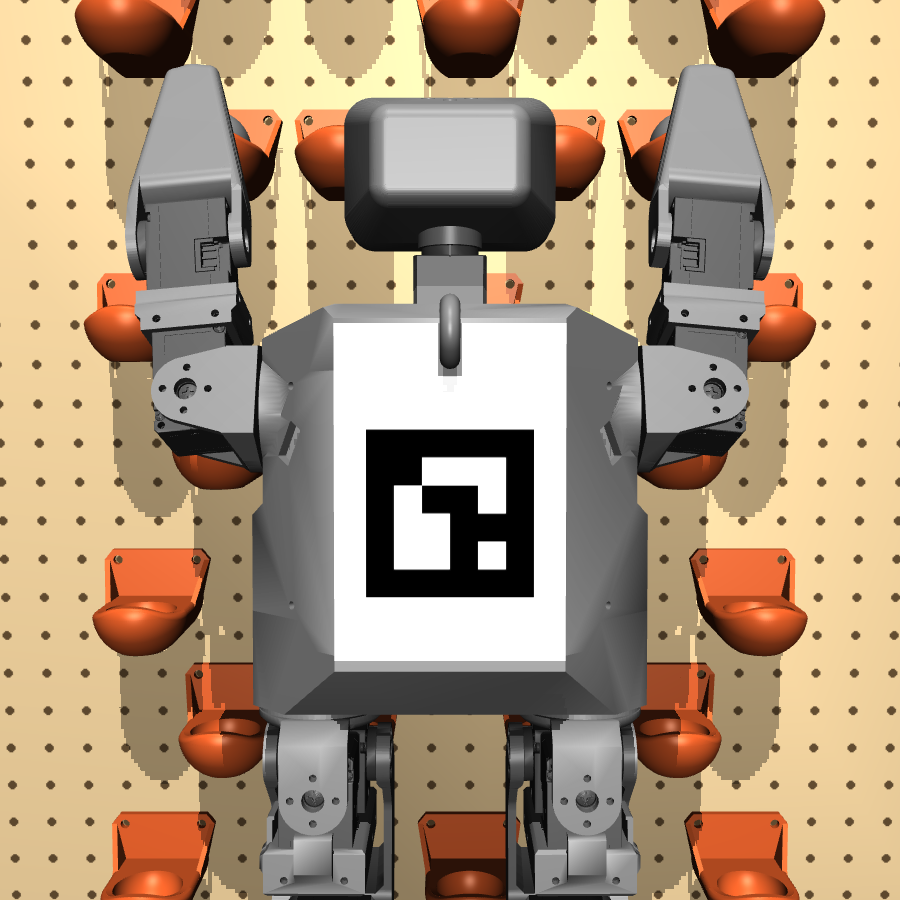
\includegraphics[width=\textwidth]{img/sticker_on_robot.png}
\caption{Sur le robot simulé.}
\end{subfigure}
\caption{Le marqueur ID~5 des organisateurs sur le dos du robot.}
\label{fig:marqueur-robot}
\end{figure}

\subsection{Le repère du marqueur dans le repère du tronc}

Pour passer de la pose du marqueur à la pose du robot, il faut savoir exactement comment le marqueur est fixé
sur le tronc. La fiche le donne ; vu de derrière le robot (comme le voient les caméras), l'axe $x_M$ va vers la
droite du robot ($-y_T$), $y_M$ vers le haut ($+z_T$), $z_M$ vers l'arrière ($-x_T$). Ces trois vecteurs sont les
colonnes de \code{R_TRUNK_MARKER}, et la position du centre du code est \code{P_TRUNK_MARKER} :
\[
  R_{TM} = \begin{pmatrix} 0 & 0 & -1 \\ -1 & 0 & 0 \\ 0 & 1 & 0 \end{pmatrix},
  \qquad
  t_{TM} = \begin{pmatrix} -33{,}0 \\ 0 \\ 54{,}75 \end{pmatrix}\text{ mm},
  \qquad
  \text{côté du code : } 42\text{ mm (\code{CODE})}.
\]

\begin{attention}[Sur le vrai robot]
Ces valeurs ne sont justes que si l'autocollant est imprimé \textbf{à 100~\%} (vérifier la règle de 100~mm et le
code de 42~mm) et collé comme le dit la fiche (encoche en butée contre le pied de la poignée, à plat). Un décalage
de quelques millimètres se retrouve tel quel dans la position du robot. S'il est collé autrement, mesurer et
corriger \code{P_TRUNK_MARKER} dans \code{robot_marker.py}.
\end{attention}

\subsection{L'ajout au simulateur : \texttt{MarkedSim}}

Le simulateur construit sa scène MuJoCo avec \code{build_spec()}. La fonction \code{add_robot_marker(spec)}
ajoute au corps \code{trunk} une boîte très fine dont la face extérieure porte l'image de l'autocollant
(\code{sticker_image()} : le code généré par OpenCV avec \code{cv2.aruco.generateImageMarker}, placé comme sur la
fiche, l'encoche en gris). Sa face est 0,3~mm devant le dos, pour être visible. La boîte est purement visuelle :
pas de collision, pas de masse.

\begin{lstlisting}[style=py]
class MarkedSim(ClimbingSim):
    """ClimbingSim with the robot's marker ID 5 on its back (same arguments)."""
    def __init__(self, *args, **kwargs):
        _sim_module.build_spec = lambda **kw: add_robot_marker(build_spec(**kw))
        try:
            super().__init__(*args, **kwargs)
        finally:
            _sim_module.build_spec = build_spec
\end{lstlisting}

\code{MarkedSim} s'utilise exactement comme \code{ClimbingSim} (\code{MarkedSim("N1")},
\code{reset_hanging()}, \code{step()}, \code{render()}\ldots). Pendant sa construction, il remplace
temporairement la fonction qui fabrique la scène par une version qui ajoute l'autocollant, puis remet
l'originale. Le dépôt du simulateur n'est pas modifié.

% =========================================================================================================
\section{Étape 3 --- Où est le robot ?}
\label{sec:robot}

\subsection{La chaîne des repères}

\begin{figure}[H]
\centering
\begin{tikzpicture}[font=\small, fr/.style={draw=accent, fill=accent!8, rounded corners=3pt, minimum width=22mm,
                    minimum height=11mm, align=center}]
  \node[fr] (W) {Mur\\$\mathcal{W}$};
  \node[fr, right=21mm of W] (C) {Caméra\\$\mathcal{C}$};
  \node[fr, right=21mm of C] (M) {Marqueur\\$\mathcal{M}$};
  \node[fr, right=21mm of M] (T) {Tronc\\$\mathcal{T}$};
  \node[fr, below=14mm of W] (S) {Monde\\MuJoCo};
  \draw[arr] (W) -- node[above, font=\footnotesize]{$R_{CW}, t_{CW}$} node[below, font=\scriptsize, align=center]{étape 1\\marqueurs 1--4} (C);
  \draw[arr] (C) -- node[above, font=\footnotesize]{détection} node[below, font=\scriptsize, align=center]{coins du\\marqueur 5} (M);
  \draw[arr] (M) -- node[above, font=\footnotesize]{$R_{TM}, t_{TM}$} node[below, font=\scriptsize, align=center]{fixe,\\fiche} (T);
  \draw[arr] (W) -- node[left, font=\footnotesize]{rotation fixe} (S);
  \draw[arr, accent, very thick] (W.south east) to[out=-25, in=-155] node[below, font=\footnotesize, text=accent]
     {résultat : $R_{WT},\ t_{WT}$ (\code{robot_pose})} (T.south west);
\end{tikzpicture}
\caption{Pour connaître la pose du tronc dans le repère du mur, on enchaîne : mur $\to$ caméra (étape 1),
caméra $\to$ marqueur (détection), marqueur $\to$ tronc (fixation donnée par la fiche).}
\label{fig:chaine}
\end{figure}

\subsection{La triangulation}

Chaque caméra calibrée transforme un pixel en un \emph{rayon} dans l'espace : le coin du marqueur est
quelque part sur ce rayon, mais une seule caméra ne dit pas à quelle distance. Avec deux caméras, le coin est
à l'\textbf{intersection des deux rayons}. C'est la triangulation (\code{cv2.triangulatePoints}, méthode
linéaire DLT), appliquée à chacun des 4 coins du marqueur ID~5.

On obtient 4 points 3D dans le repère du mur. On connaît aussi la forme du marqueur (un carré de 42~mm,
\code{square_corners(0.042)}). Il reste à trouver la rotation et la translation qui superposent au mieux le
carré théorique sur les 4 points mesurés : c'est l'\textbf{algorithme de Kabsch} (\code{_rigid_fit}), qui
résout ce problème exactement avec une décomposition en valeurs singulières :
\[
  H = \sum_i (a_i - \bar a)(b_i - \bar b)^\top = U \Sigma V^\top,
  \qquad
  R = V \,\mathrm{diag}\bigl(1, 1, \det(V U^\top)\bigr)\, U^\top,
  \qquad
  t = \bar b - R\,\bar a,
\]
où $a_i$ sont les coins du carré théorique et $b_i$ les coins triangulés. Le $\det$ garantit une vraie
rotation (pas un miroir).

\subsection{Deux caméras obligatoires}

Avec une seule caméra, la distance du marqueur ne peut venir que de sa \emph{taille apparente} dans l'image.
Avec une focale $f$ (1386~pixels pour une D435i en 1920~×~1080, 924 en 1280~×~720), un marqueur de $L = 42$~mm à
$Z \approx 2{,}4$~m fait $s = fL/Z \approx 24$~pixels (16 en 1280~×~720). Une erreur $\delta s$ sur sa taille
donne une erreur de profondeur
\[
  \delta Z_{\text{1 caméra}} \approx \frac{Z^2}{f\,L}\,\delta s \approx \frac{2{,}4^2}{1386 \times 0{,}042}
  \times 0{,}25 \approx 2{,}5~\text{cm}
  \qquad\text{(3,7 cm en 1280~×~720, pour } \delta s \approx 0{,}25 \text{ pixel)}.
\]
Avec deux caméras écartées de $B \approx 1{,}1$~m, c'est l'écartement qui remplace la taille du marqueur :
\[
  \delta Z_{\text{2 caméras}} \approx \frac{Z^2}{f\,B}\,\delta d \approx \frac{2{,}4^2}{1386 \times 1{,}1}
  \times 0{,}25 \approx 1~\text{mm}.
\]
Le \code{Tracker} n'accepte donc la pose du robot que si \textbf{les deux caméras} voient son marqueur
(\code{min_views = 2}) ; sinon \code{update()} renvoie \code{None}. Avant cette règle, les rares images vues par
une seule caméra donnaient des erreurs jusqu'à \textbf{12~cm}.

\begin{figure}[H]
\centering
\begin{subfigure}[b]{0.45\textwidth}
\centering
\begin{tikzpicture}[font=\footnotesize, scale=0.95]
  \fill[wallc] (-2.2,4.3) rectangle (2.2,4.55);
  \node[brown!50!black] at (0,4.75) {mur (vue de dessus)};
  \fill[black] (0,0) ++(-0.2,-0.12) rectangle ++(0.4,0.24);
  \node[below=2pt] at (0,-0.12) {caméra};
  \draw[orange!80!black] (0,0) -- (-0.11,4.1) (0,0) -- (0.11,4.1);
  \fill[okgreen!35, draw=okgreen] (0,3.9) ellipse (0.13 and 0.62);
  \fill[black] (-0.12,3.9) rectangle (0.12,3.94);
  \node[align=left, anchor=west] at (0.4,3.6) {incertitude\\$\approx$ 2,5 cm en\\profondeur};
  \draw[<->] (-1.5,0) -- (-1.5,3.9) node[midway, left] {$Z \approx 2{,}4$ m};
\end{tikzpicture}
\caption{Une caméra : la distance vient de la \emph{taille apparente} du marqueur (environ 24~pixels),
mesure peu précise.}
\end{subfigure}\hfill
\begin{subfigure}[b]{0.5\textwidth}
\centering
\begin{tikzpicture}[font=\footnotesize, scale=0.95]
  \fill[wallc] (-2.4,4.3) rectangle (2.4,4.55);
  \node[brown!50!black] at (0,4.75) {mur (vue de dessus)};
  \foreach \cx in {-1.6,1.6}{
    \fill[black] (\cx,0) ++(-0.2,-0.12) rectangle ++(0.4,0.24);
    \draw[orange!80!black] (\cx,0) -- ($(\cx,0)!1.05!(-0.035,3.9)$) (\cx,0) -- ($(\cx,0)!1.05!(0.035,3.9)$);}
  \fill[okgreen!35, draw=okgreen] (0,3.9) ellipse (0.06 and 0.1);
  \node[below=2pt] at (-1.6,-0.12) {gauche};
  \node[below=2pt] at (1.6,-0.12) {droite};
  \draw[<->] (-1.6,-0.65) -- (1.6,-0.65) node[midway, below] {$B \approx 1{,}1$ m};
  \node[align=left, anchor=west] at (0.35,3.55) {incertitude\\$\approx$ 1 mm};
\end{tikzpicture}
\caption{Deux caméras : la position est à l'intersection des rayons ; l'écart $B$ entre les caméras rend la
mesure de profondeur précise.}
\end{subfigure}
\caption{Pourquoi deux caméras valent beaucoup mieux qu'une.}
\label{fig:triangulation}
\end{figure}

\subsection{Le petit marqueur : 1920 × 1080}

Le code de 42~mm est petit : vu à 2,4~m, il fait environ 16~pixels de côté en 1280~×~720, moins de 3~pixels par
case. En \textbf{1920~×~1080} (une résolution de la D435i), il en fait 24 : les coins sont mieux placés, et le
marqueur est vu plus souvent par les deux caméras. C'est la résolution par défaut de \code{demo.py} et de
\code{live.py} (tableau~\ref{tab:reglages}).

\subsection{L'inclinaison par l'IMU : \texttt{level\_with\_gravity()}}

Les coins d'un marqueur de 42~mm, placés au millimètre près, laissent une incertitude d'orientation de l'ordre de
$1/21$~rad, soit 2 à 3°. Or le centre du marqueur est à $\sqrt{33^2 + 54{,}75^2} \approx 64$~mm de l'origine du
tronc : 3° d'erreur d'orientation déplacent l'origine du tronc de $64 \times 0{,}05 \approx 3$~mm.

Le robot a une centrale inertielle (IMU) qui mesure la direction de la gravité dans son repère
(\code{obs["gravity"]}), bien plus précisément. Elle donne l'\emph{inclinaison} du robot, mais pas son \emph{cap}
(sa rotation autour de la verticale) : l'IMU ne sait pas où est le mur. On combine donc les deux :
\begin{enumerate}
  \item avec l'orientation $R$ donnée par le marqueur, la gravité mesurée par l'IMU ($g_T$, repère du tronc) devrait
        pointer vers le bas du mur : $v = R\,g_T$ devrait valoir $d = (0, -1, 0)$ ;
  \item on calcule la plus petite rotation $Q$ qui amène $v$ sur $d$ (axe $v \times d$, angle entre $v$ et $d$), et on
        corrige : $R' = Q\,R$ ; le cap du marqueur est conservé, l'inclinaison vient de l'IMU ;
  \item le centre $c$ du marqueur, bien mesuré par la triangulation, ne bouge pas ; l'origine du tronc suit :
        $t' = c - R'\,t_{TM}$.
\end{enumerate}

\begin{lstlisting}[style=py]
pose = tracker.update(images, obs["gravity"])     # marqueur + inclinaison de l'IMU
pose = tracker.update(images)                     # marqueur seul
\end{lstlisting}

Résultat : l'erreur moyenne passe de 2,4~mm à \textbf{0,9~mm} (mur N2, caméras par défaut, 1920~×~1080).

\subsection{Du marqueur au tronc : \texttt{robot\_pose()}}

La triangulation donne la pose du marqueur dans le repère du mur, $(R_{WM}, t_{WM})$. Le marqueur étant fixé
sur le tronc par $(R_{TM}, t_{TM})$, on inverse cette fixation :
\[
  R_{WT} = R_{WM}\,R_{TM}^\top,
  \qquad
  t_{WT} = t_{WM} - R_{WT}\,t_{TM}.
\]
Enfin \code{to_world(R, p)} convertit cette pose dans le repère du simulateur, pour la comparer à la vérité
(\code{sim.trunk_pose()}) ou pour la donner au programme de grimpe.

% =========================================================================================================
\section{Étape 4 --- Où sont les prises ?}
\label{sec:prises}

\subsection{L'idée}

Les prises ne sont pas n'importe où : elles sont boulonnées sur la grille de 52~×~93 trous du mur, au pas de
15~mm, chacune sur deux trous voisins d'une même rangée. Une prise est donc désignée par sa \emph{colonne} et sa
\emph{rangée} (celles de son trou de gauche), et il n'y a qu'environ 4\,600 places possibles. On connaît aussi sa
forme exacte : le modèle 3D de la vraie prise est fourni avec le simulateur. Plutôt que de chercher des taches
de couleur au hasard dans l'image, on \textbf{essaie chaque place} : on projette dans chaque image la prise qui
serait là, et on regarde si elle tombe sur de la couleur.

\begin{figure}[H]
\centering
\begin{tikzpicture}[node distance=6mm and 8mm]
  \node[box=gray] (img) {images des caméras\\\footnotesize (calibrées, étape 1)};
  \node[box=accent, right=of img] (cls) {\code{pixel_classes()}\\\footnotesize prise / mur / inconnu};
  \node[box=gray, below=of img] (cand) {\code{hold_candidates()}\\\footnotesize les $\approx$ 4\,600 places};
  \node[box=gray, below=of cand] (pts) {\code{hold_points()}\\\footnotesize 200 points de la prise};
  \node[box=orange, right=of cand, yshift=-8mm] (px) {\code{hold_pixels()}\\\footnotesize où tombe chaque place\\(une fois par calibration)};
  \node[box=okgreen, right=of px] (votes) {\code{hold_votes()}\\\footnotesize compte les points\\colorés et visibles};
  \node[box=okgreen, above=of votes] (acc) {cumul des votes\\\footnotesize au fil des images};
  \node[box=purple, below=of votes] (sel) {\code{select_holds()}\\\footnotesize meilleures places,\\sans chevauchement};
  \draw[arr] (img) -- (cls);
  \draw[arr] (cand) -- (px);
  \draw[arr] (pts) -| (px);
  \draw[arr] (cls) -| (votes);
  \draw[arr] (px) -- (votes);
  \draw[arr] (votes) -- (acc);
  \draw[arr] (votes) -- (sel);
\end{tikzpicture}
\caption{La détection des prises (\code{Tracker.find_holds()}).}
\end{figure}

\subsection{Classer les pixels}

Chaque pixel est rangé dans une de trois classes, d'après sa \emph{saturation} (la vivacité de la couleur, 0 à
255) et sa \emph{luminosité} (0 à 255), quelle que soit sa teinte :

\begin{center}
\renewcommand{\arraystretch}{1.2}
\begin{tabularx}{\textwidth}{l l X}
\toprule
Classe & Règle & Ce que c'est \\
\midrule
\textbf{prise} & saturation $\geq 120$ & une couleur vive : vert, orange, bleu\ldots{} (toutes les prises) \\
\textbf{mur} & saturation entre 10 et 120 & une couleur pâle : le contreplaqué (15--40 sur le vrai mur, 67 dans le simulateur) \\
\textbf{inconnu} & saturation $< 10$ ou luminosité $< 50$ & gris, blanc, noir : le robot, les marqueurs, les ombres et les trous \\
\bottomrule
\end{tabularx}
\end{center}

La classe « inconnu » est essentielle : un pixel du robot \emph{cache} peut-être une prise ; il ne doit compter ni pour
ni contre. Le seuil de 10 a été fixé après un essai sur la photo du vrai mur : avec un seuil de 40, le contreplaqué
réel, presque blanc, était classé « inconnu » (figure~\ref{fig:reel}).

\subsection{Le score d'une place}

Pour chaque place possible, on prend \textbf{200 points} répartis uniformément sur la surface du modèle 3D de la prise
(\code{hold_points()}), on les place à cet endroit du mur et on les projette dans l'image de chaque caméra. Même les
points cachés (derrière la coupelle) tombent sur la prise dans l'image : la prise entière doit donc être colorée. On
compte les points qui tombent sur un pixel « prise » ($h$), sur un pixel connu, « prise » ou « mur » ($k$), et dans
l'image ($n$). Ces comptes s'additionnent sur les caméras. Alors :
\[
  \text{score} = \frac{h}{k} \quad\text{(la part visible qui est colorée)},
  \qquad
  \text{vu} = \frac{k}{n} \quad\text{(la part visible, non cachée)}.
\]
Une place est une prise si \textbf{score $\geq 0{,}8$} et \textbf{vu $\geq 0{,}4$}. Ces seuils ont été choisis sur
12 cas du simulateur (3 murs, 4 placements de caméras, robot devant le mur, une seule image) :

\begin{center}
\begin{tabular}{lcc}
\toprule
Seuils (vu / score) & Fausses prises & Prises manquées (cachées par le robot) \\
\midrule
0,3 / 0,7 & 19 & 65 \\
0,3 / 0,8 & 7 & 70 \\
\textbf{0,4 / 0,8 (choisi)} & \textbf{2} & \textbf{99} \\
0,5 / 0,8 & 2 & 121 \\
0,6 / 0,8 & 3 & 147 \\
\bottomrule
\end{tabular}
\end{center}
(sur 984 prises au total.) Une fausse prise est bien plus dangereuse qu'une prise manquée (le robot tendrait la main
dans le vide) ; et les prises manquées sont retrouvées par le cumul des images (section~\ref{sec:cumul}).

\subsection{Choisir les prises}

Les places sont prises de la meilleure à la moins bonne, en sautant celles dont la prise chevaucherait une prise déjà
choisie (deux prises ne peuvent pas être boulonnées là ; le simulateur fournit cette règle, \code{OVERLAP}).

\paragraph{Deux prises collées.} Deux prises côte à côte (à 45~mm, le plus près possible) forment une seule tache de
couleur. Le score forme alors un \emph{plateau} sur toute la largeur de la tache, avec souvent son maximum au
\emph{milieu}, entre les deux prises (figure~\ref{fig:plateau}) : choisir ce milieu bloquerait les deux vraies
places. Après le premier choix, chaque prise choisie est donc remplacée par \textbf{deux} prises voisines si elles
expliquent mieux la tache : chacune doit avoir un score $\geq 0{,}7$, et la somme de leurs excès au-dessus de 0,7
doit dépasser celui de la prise seule. Une prise isolée ne peut pas déclencher cet échange : une place décalée de
30~mm ne couvre qu'une petite partie de la prise.

\begin{figure}[H]
\centering
\begin{tikzpicture}[x=0.62cm, y=4cm, font=\footnotesize]
  \fill[okgreen!8] (2.6,0) rectangle (6.4,1.02);
  \fill[okgreen!8] (10.6,0) rectangle (14.4,1.02);
  \draw[->] (-0.5,0) -- (18,0) node[right] {colonne};
  \draw[->] (-0.5,0) -- (-0.5,1.1) node[above] {score};
  \foreach \y in {0,0.5,1}{\draw (-0.6,\y) -- (-0.4,\y) node[left=2pt] {\y};}
  \draw[dashed, axx] (-0.5,0.8) -- (17.5,0.8) node[right] {0,8};
  \draw[dotted, holdc, thick] (-0.5,0.7) -- (17.5,0.7) node[right] {0,7};
  \foreach \c/\s [count=\i from 0] in {15/0.04,16/0.26,17/0.57,18/0.81,19/0.86,20/0.90,21/0.83,22/0.61,23/0.33,
                                       24/0.35,25/0.56,26/0.80,27/0.88,28/0.91,29/0.84,30/0.61,31/0.33,32/0.10}{
    \fill[accent!70] (\i-0.3,0) rectangle (\i+0.3,\s);
    \node[below, font=\scriptsize] at (\i,0) {\c};}
  \foreach \i in {5,13}{\node[axx, font=\small] at (\i,0.98) {$\times$};}
  \foreach \i in {3,6,11,14}{\node[okgreen, font=\small] at (\i,1.06) {$\blacktriangledown$};}
  \node[anchor=west, align=left] at (19.0,0.45) {\textcolor{axx}{$\times$} choix naïf\\(le milieu)\\
        \textcolor{okgreen}{$\blacktriangledown$} après\\l'échange :\\les 4 prises};
\end{tikzpicture}
\caption{Le score le long d'une rangée de la photo du vrai mur (rangée 9). Les deux paires de prises (colonnes 18 et
21, 26 et 29) forment deux plateaux dont le maximum est au milieu (20 et 28). L'échange « une prise $\to$ deux »
retrouve les quatre vraies prises.}
\label{fig:plateau}
\end{figure}

\subsection{Le cumul au fil des images}
\label{sec:cumul}

Les prises ne bougent pas. Chaque appel à \code{tracker.find_holds(images)} \emph{ajoute} les comptes $h$ et $k$ des
nouvelles images à ceux des précédentes, et garde pour chaque place la meilleure part vue sur une image. Une prise
cachée par le robot à un instant compte dès qu'elle apparaît : quand le robot monte, celles qu'il cachait en bas
redeviennent visibles. \code{reset_holds()} oublie tout (quand les prises ont été déplacées).

La projection des 4\,600~×~200 points ne dépend que de la pose des caméras : elle est faite une fois par
calibration (0,3 à 0,6~s), et chaque nouvelle image ne coûte ensuite qu'environ \textbf{10~ms}.

\subsection{La couleur, et le résultat}

La couleur de chaque prise est la teinte moyenne de ses pixels vifs (moyenne sur un cercle, le rouge étant aux deux
bouts de l'échelle des teintes), nommée : rouge, orange, jaune, vert, bleu, violet.

\code{find_holds()} renvoie une liste de prises (\code{FoundHold}), de la plus basse à la plus haute :
\begin{itemize}
  \item \code{f.hold.col}, \code{f.hold.row} : sa place sur la grille ;
  \item \code{f.hold.socket} : le centre de sa coupelle (là où se pose la boule du robot), \textbf{repère du monde}, en
        mètres ; \code{f.socket_wall} : le même point dans le repère du mur ;
  \item \code{f.color}, \code{f.score}, \code{f.seen}.
\end{itemize}
\code{demo.py} et \code{live.py} les enregistrent dans \code{out/holds.json}, un fichier de mur du simulateur :
on peut l'ouvrir dans l'éditeur de mur (\code{climbing-sim-wall-editor}) ou y accrocher le robot.

% =========================================================================================================
\section{Tout ensemble : la classe Tracker}

\begin{figure}[H]
\centering
\begin{tikzpicture}[node distance=7mm and 8mm]
  \node[box=gray] (imgL) {image caméra gauche};
  \node[box=gray, right=of imgL] (imgR) {image caméra droite};
  \node[box=accent, below=of $(imgL)!0.5!(imgR)$] (det) {\code{detect()}\\\footnotesize marqueurs et coins};
  \node[box=orange, below=10mm of det, xshift=-24mm] (cam) {\code{camera_pose()}\\\footnotesize IDs 1--4 $\to$ pose des caméras};
  \node[box=okgreen, below=10mm of det, xshift=24mm] (m5) {coins du marqueur ID~5\\\footnotesize les deux caméras};
  \node[box=okgreen, below=of m5] (tri) {\code{marker_pose()}\\\footnotesize triangulation + Kabsch};
  \node[box=okgreen, below=of tri] (rp) {\code{robot_pose()}\\\footnotesize pose du tronc (mur)};
  \node[box=gray, right=6mm of rp, text width=20mm] (imu) {IMU\\\footnotesize gravité};
  \node[box=okgreen, below=of rp] (lev) {\code{level_with_gravity()}\\\footnotesize inclinaison par l'IMU};
  \node[box=holdc, below=of cam] (holds) {\code{find_holds()}\\\footnotesize les prises};
  \node[box=purple, below=of lev] (tw) {\code{to_world()}\\\footnotesize repère du simulateur};
  \node[box=gray, below=of tw, dashed] (plan) {programme de grimpe\\\footnotesize (à venir)};
  \draw[arr] (imgL) -- (det);
  \draw[arr] (imgR) -- (det);
  \draw[arr] (det) -- (cam);
  \draw[arr] (det) -- (m5);
  \draw[arr] (cam.east) -- ++(4mm,0) |- (tri.west);
  \draw[arr] (cam) -- (holds);
  \draw[arr] (m5) -- (tri);
  \draw[arr] (tri) -- (rp);
  \draw[arr] (rp) -- (lev);
  \draw[arr] (imu) |- (lev);
  \draw[arr] (lev) -- (tw);
  \draw[arr, dashed] (tw) -- (plan);
  \draw[arr, dashed] (holds) |- (plan);
  \begin{scope}[on background layer]
    \node[fit=(cam)(holds), fill=orange!6, draw=orange!60, rounded corners, inner sep=3mm,
          label={[font=\footnotesize\sffamily, text=orange!70!black, align=center]left:\code{calibrate()}\\+ prises}] {};
    \node[fit=(m5)(tri)(rp)(lev), fill=okgreen!5, draw=okgreen!60, rounded corners, inner sep=3mm] {};
  \end{scope}
\end{tikzpicture}
\caption{Le traitement complet. La calibration des caméras et la recherche des prises (orange) se font au début de
chaque essai, puis les prises sont complétées au fil des images ; le suivi du robot (vert, \code{update()}) se fait à
chaque nouvelle image.}
\label{fig:pipeline}
\end{figure}

\begin{lstlisting}[style=py]
from perception import Tracker, to_world
from robot_marker import CODE, R_TRUNK_MARKER, P_TRUNK_MARKER

tracker = Tracker({"cam_left": K_gauche, "cam_right": K_droite},   # intrinseques
                  CODE, R_TRUNK_MARKER, P_TRUNK_MARKER)
images = {"cam_left": img_g, "cam_right": img_d}
tracker.calibrate(images)                  # debut d'essai : pose des cameras
holds = tracker.find_holds(images)         # les prises (puis de temps en temps)
pose = tracker.update(images, obs["gravity"])   # a chaque image ; None si une camera
if pose is not None:
    R, p = pose                            # tronc, repere du mur (p en metres)
    R_monde, p_monde = to_world(R, p)
for f in holds:
    print(f.hold.col, f.hold.row, f.color, f.hold.socket)   # socket : repere du monde
\end{lstlisting}

% =========================================================================================================
\section{Les programmes et leurs commandes}

Toutes les commandes se lancent depuis \code{~/Desktop/Hackathon/simulator} (pour que \code{uv} utilise
l'environnement du simulateur), avec \code{--with opencv-contrib-python} pour ajouter OpenCV.

\subsection{\texttt{demo.py} --- la démonstration dans le simulateur}

\begin{lstlisting}[style=sh]
uv run --with opencv-contrib-python python ../perception/demo.py [N1|N2|N3] [--shuffle SEED] [--res WxH] [--show]
\end{lstlisting}

\begin{center}
\renewcommand{\arraystretch}{1.2}
\begin{tabularx}{\textwidth}{l X}
\toprule
Option & Effet \\
\midrule
\code{N1}, \code{N2}, \code{N3} & le mur (niveaux de difficulté 1 à 3 du règlement) ; \code{N1} par défaut \\
\code{--shuffle SEED} & place les deux caméras au hasard devant le mur : entre 1,9 et 3~m du mur, entre
0,5 et 1,4~m de haut, une de chaque côté, visée près du centre ; un placement est retiré tant qu'une caméra
ne voit pas les quatre coins. \code{SEED} (un entier) choisit le tirage. \\
\code{--res WxH} & la taille des images des caméras, une résolution de la D435i : \code{1920x1080} par défaut,
\code{1280x720} pour comparer \\
\code{--show} & une fenêtre montre les caméras pendant la démonstration ; à la fin, une touche la ferme \\
\bottomrule
\end{tabularx}
\end{center}

\paragraph{Ce que fait le script.}
\begin{enumerate}
  \item Il crée la simulation avec l'autocollant (\code{MarkedSim}) et accroche le robot à ses quatre prises de
        départ (\code{reset_hanging}).
  \item \textbf{Les caméras} : il calibre les caméras et compare la pose trouvée à leur vraie pose.
  \item \textbf{Les prises} : il les cherche, les compare aux prises du mur, en affiche quelques-unes avec leur
        position, et les écrit dans \code{out/holds.json}.
  \item \textbf{Le robot} : pendant 3~secondes simulées (151 pas de 20~ms), il fait se balancer le robot (le tronc
        oscille de ±30~mm de côté et ±15~mm en hauteur, mains et pieds dans leurs prises). À chaque pas, il prend les
        deux images, calcule la pose du tronc avec le marqueur seul et avec l'IMU, et la compare à la vraie.
  \item Il enregistre la \textbf{vidéo} \code{out/demo.mp4} (figure~\ref{fig:video}), et des images annotées et
        brutes (\code{cam_left.png}, \code{cam_left_raw.png}\ldots).
\end{enumerate}

\paragraph{Lire la sortie.} Voici ce qu'affiche \code{demo.py N2} (extraits) :

\begin{figure}[H]
\begin{lstlisting}[style=out]
cam_left at x -0.15 m, 0.90 m high, 2.40 m from the wall, 1920 x 1080 pixels
  cam_left: markers [1, 2, 3, 4, 5], reprojection 0.38 px, position error 1.8 mm, angle error 0.019 deg
holds from their colour (ground truth: the 88 holds of wall N2): found 81, correct 81, false 0, missed 7 (hidden behind the robot)
  col 18 row  2 orange  socket: world [302 -26  26] mm = on the wall x 302 mm, height 26 mm  (ok)
  all of them: /Users/.../Hackathon/perception/out/holds.json
trunk pose from marker ID 5, with the IMU's tilt (ground truth: the simulated trunk)
  t= 1.02 s: trunk at [ 386 -116  172] mm (true [ 385 -116  172]), error  0.7 mm 1.13 deg (marker alone:  6.4 mm)
marker alone  : mean error 2.4 mm (max 7.5), 2.33 deg (max 6.80) over 151 images
marker + IMU  : mean error 0.9 mm (max 3.0), 1.18 deg (max 5.33) over 151 images
0 of 151 images not used: the robot's marker seen by one camera only
video: /Users/.../Hackathon/perception/out/demo.mp4
\end{lstlisting}
\end{figure}

\begin{center}
\renewcommand{\arraystretch}{1.2}
\begin{tabularx}{\textwidth}{>{\raggedright}p{4.4cm} X}
\toprule
Ligne & Signification \\
\midrule
\code{cam_left at x ...} & où le simulateur a placé la caméra (la vérité, que le code ne connaît pas) \\
\code{markers [1, 2, 3, 4, 5]} & les marqueurs détectés dans l'image : il faut 1--4 (coins) et 5 (robot) \\
\code{reprojection 0.38 px} & écart moyen entre les coins détectés et les coins reprojetés : < 1 pixel = bon \\
\code{position error 1.8 mm} & distance entre la position calculée de la caméra et la vraie \\
\code{found 81, correct 81, false 0} & prises trouvées, justes, fausses ; \code{missed} : cachées par le robot \\
\code{socket: world [x y z]} & centre de la coupelle de la prise, repère du monde ; \code{on the wall} : repère du mur \\
\code{trunk at [x y z] mm} & position du tronc calculée par les caméras (avec l'IMU), repère du monde \\
\code{(true [x y z])} & la vraie position dans le simulateur \\
\code{error 0.7 mm 1.13 deg} & écart de position et d'orientation ; \code{marker alone} : sans l'IMU \\
\code{images not used} & images où une seule caméra voyait le marqueur du robot (pose refusée) \\
\bottomrule
\end{tabularx}
\end{center}

\begin{figure}[H]
\centering
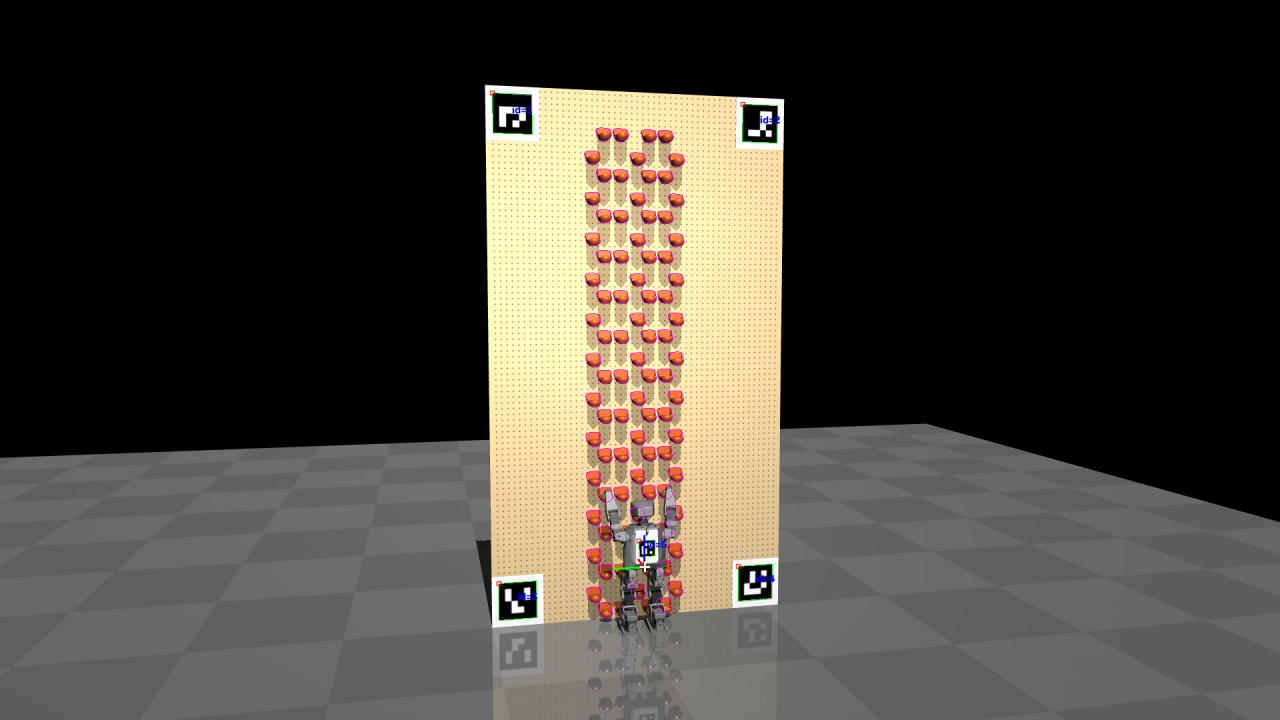
\includegraphics[width=0.49\textwidth]{img/cam_left_annotated.png}\hfill
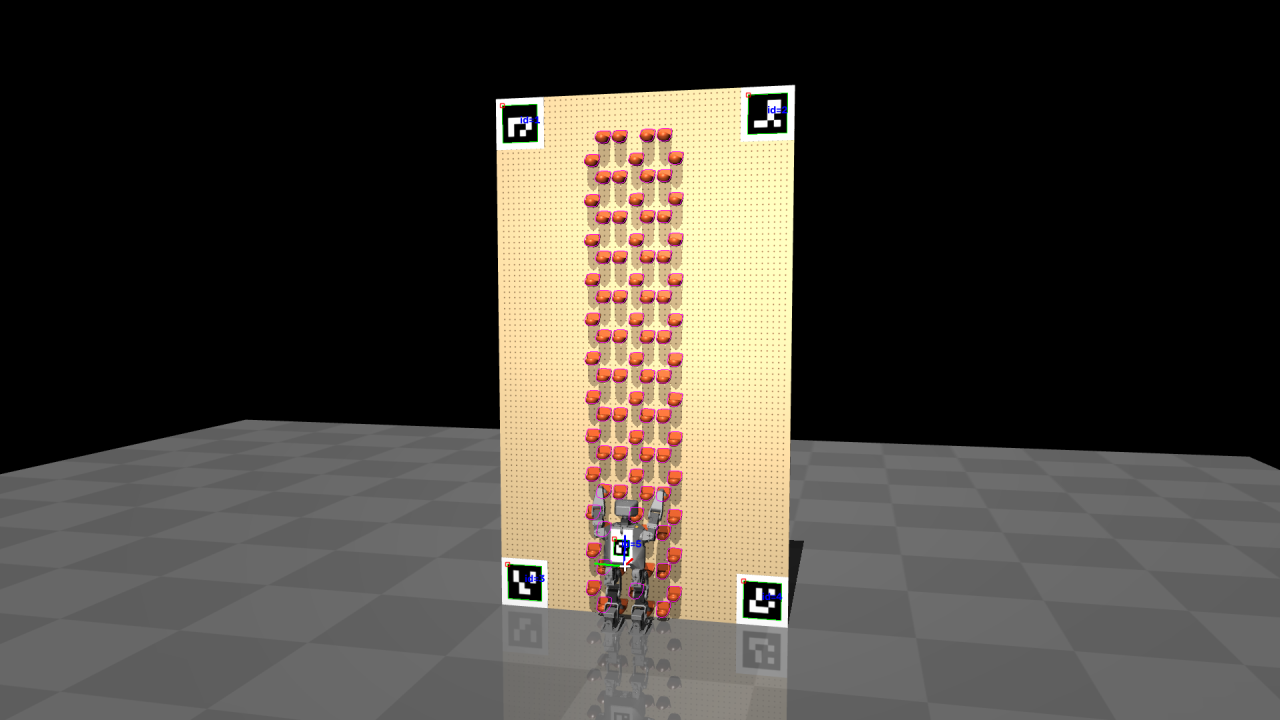
\includegraphics[width=0.49\textwidth]{img/cam_right_annotated.png}\\[2mm]
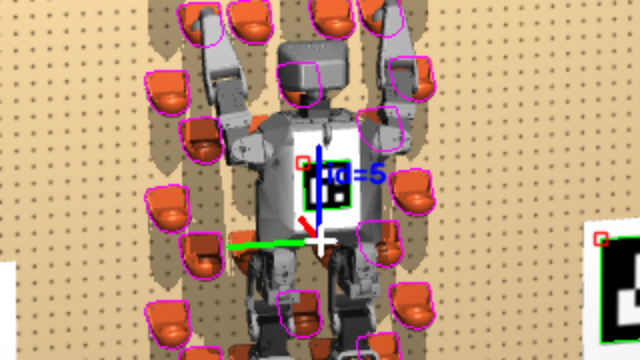
\includegraphics[width=0.49\textwidth]{img/cam_left_zoom.png}\hfill
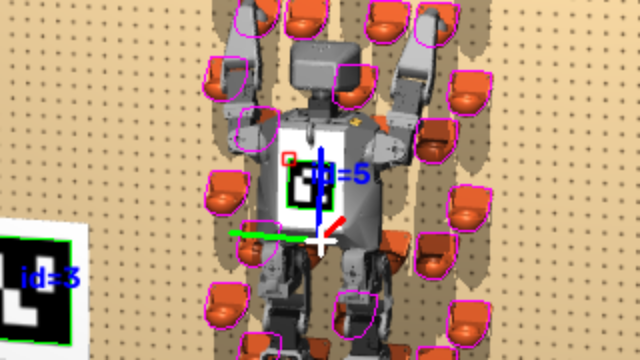
\includegraphics[width=0.49\textwidth]{img/cam_right_zoom.png}
\caption{Ce que montrent la fenêtre \code{--show} et la vidéo \code{demo.mp4} : les deux caméras (en haut) et un zoom
sur le robot (en bas). En vert, les marqueurs détectés ; en magenta, le contour des prises trouvées ; les flèches
rouge, verte et bleue : le repère du tronc calculé par les caméras ; la croix blanche : la vraie position du tronc.
Les flèches doivent partir de la croix.}
\label{fig:video}
\end{figure}

\subsection{\texttt{live.py} --- le jour J (vraies caméras ou images)}

\begin{lstlisting}[style=sh]
# deux cameras USB, gauche puis droite
uv run --with opencv-contrib-python python ../perception/live.py 0 1
# avec la calibration des cameras
uv run --with opencv-contrib-python python ../perception/live.py 0 1 --cameras cams.json
# sur deux images (ici les images brutes laissees par la demo), sans fenetre
uv run --with opencv-contrib-python python ../perception/live.py \
    ../perception/out/cam_left_raw.png ../perception/out/cam_right_raw.png --once
\end{lstlisting}

\begin{center}
\renewcommand{\arraystretch}{1.2}
\begin{tabularx}{\textwidth}{l X}
\toprule
Argument & Effet \\
\midrule
\code{0 1} (sources) & une ou deux sources, \textbf{la caméra gauche en premier} : un numéro de caméra USB ou un
fichier image. Une RealSense apparaît comme plusieurs caméras (couleur, infrarouge\ldots) : essayer 0, 1, 2\ldots{}
jusqu'à voir l'image couleur. \\
\code{--size 1920x1080} & la taille d'image demandée aux caméras (par défaut 1920~×~1080, pour le petit marqueur
du robot) \\
\code{--cameras cams.json} & la calibration de chaque caméra (\code{fx}, \code{fy}, \code{cx}, \code{cy}, et
facultativement \code{dist}, les coefficients de distorsion d'OpenCV). Sans ce fichier : les valeurs théoriques
de la D435i (moins précis). \\
\code{--once} & une seule image par caméra, pas de fenêtre : affiche la liste des prises et la position du robot,
enregistre \code{out/holds.json} et les images annotées \\
\bottomrule
\end{tabularx}
\end{center}

\paragraph{Les touches dans la fenêtre.} \textbf{c} : recalibrer les caméras et rechercher les prises (au début de
chaque essai, de préférence \emph{avant} de mettre le robot sur le mur) ; \textbf{h} : afficher la liste des prises dans
le terminal et l'écrire dans \code{out/holds.json} ; \textbf{s} : sauvegarder les images annotées ; \textbf{q} : quitter.

\begin{figure}[H]
\centering
\begin{tikzpicture}[node distance=5mm, font=\small]
  \node[box=gray] (open) {ouvrir les sources\\\footnotesize caméras USB ou images};
  \node[box=gray, below=of open] (intr) {intrinsèques\\\footnotesize \code{--cameras} ou D435i};
  \node[box=orange, below=of intr] (cal) {\code{calibrate()}\\\footnotesize caméras + prises};
  \node[box=okgreen, below=of cal] (upd) {\code{update()}, \code{find_holds()}\\\footnotesize robot, prises (cumul)};
  \node[box=accent, below=of upd] (show) {affichage annoté\\\footnotesize robot en mm, nombre de prises};
  \node[box=gray, below=of show] (read) {lire les images suivantes};
  \node[box=gray, right=14mm of show, text width=30mm] (keys) {touche ?\\\footnotesize c : recalibrer\\h : liste des prises\\s : sauvegarder\\q : quitter};
  \draw[arr] (open) -- (intr);
  \draw[arr] (intr) -- (cal);
  \draw[arr] (cal) -- (upd);
  \draw[arr] (upd) -- (show);
  \draw[arr] (show) -- (read);
  \draw[arr] (show) -- (keys);
  \draw[arr] (keys) |- node[pos=0.25, right, font=\scriptsize]{c} (cal);
  \draw[arr] (read.west) -- ++(-8mm,0) |- (upd.west);
\end{tikzpicture}
\caption{La boucle de \code{live.py}.}
\end{figure}

La ligne d'état indique par exemple :
\begin{lstlisting}[style=out]
robot: x    391 mm, height    172 mm,   116 mm from the wall, seen by ['cam_left', 'cam_right']
robot: marker seen by cam_left only (both cameras needed: one is centimetres off)
\end{lstlisting}
Les positions sont dans le \textbf{repère du mur} : $x$ depuis le bord gauche, hauteur depuis le bas, distance au mur.
Avec \textbf{h}, la liste des prises :
\begin{lstlisting}[style=out]
81 holds, from the bottom up (grid column and row; their socket: x from the wall's left edge, height from its bottom):
  col 18 row  2  orange  x  302 mm, height    26 mm
  col 21 row  2  orange  x  348 mm, height    26 mm
\end{lstlisting}

\subsection{\texttt{doc/make\_figures.py}}

Régénère les images de ce document à partir du simulateur (\code{perception/doc/img/}). Le document se compile
avec \code{latexmk -xelatex perception_aruco.tex} dans \code{perception/doc/}.

% =========================================================================================================
\section{Comment tester}
\label{sec:tester}

\begin{enumerate}
  \item \textbf{La démonstration, avec la fenêtre.}
\begin{lstlisting}[style=sh]
cd ~/Desktop/Hackathon/simulator
uv run --with opencv-contrib-python python ../perception/demo.py N2 --show
\end{lstlisting}
  Elle dure environ 30~secondes ; à la fin, cliquer dans la fenêtre et appuyer sur une touche. C'est réussi si :
  chaque caméra voit \code{[1, 2, 3, 4, 5]} avec une reprojection sous 1~pixel ; \code{false 0} pour les prises ;
  \code{marker + IMU : mean error} autour de 1~mm ; peu ou pas d'images inutilisées ; dans la fenêtre, les flèches
  partent de la croix blanche.

  \item \textbf{La vidéo}, à revoir autant qu'on veut :
\begin{lstlisting}[style=sh]
open ../perception/out/demo.mp4
\end{lstlisting}

  \item \textbf{Les autres murs, d'autres placements de caméras, l'autre résolution} :
\begin{lstlisting}[style=sh]
uv run --with opencv-contrib-python python ../perception/demo.py N3
uv run --with opencv-contrib-python python ../perception/demo.py N2 --shuffle 3
uv run --with opencv-contrib-python python ../perception/demo.py N2 --res 1280x720
\end{lstlisting}

  \item \textbf{Les prises trouvées}, dans l'éditeur de mur du simulateur (dans le navigateur) :
\begin{lstlisting}[style=sh]
uv run climbing-sim-wall-editor ../perception/out/holds.json
\end{lstlisting}

  \item \textbf{Le script du jour J sur des images} (sans caméra), avec les images brutes laissées par la démo :
\begin{lstlisting}[style=sh]
uv run --with opencv-contrib-python python ../perception/live.py \
    ../perception/out/cam_left_raw.png ../perception/out/cam_right_raw.png --once
\end{lstlisting}
\end{enumerate}

% =========================================================================================================
\section{Résultats}
\label{sec:resultats}

Toutes les mesures du simulateur comparent la sortie du code à la vérité du simulateur. La simulation est
déterministe : les mêmes commandes redonnent exactement les mêmes chiffres.

\subsection{Pose des caméras}

\begin{center}
\begin{tabular}{lcccc}
\toprule
Caméra (1920~×~1080) & Marqueurs vus & Reprojection & Erreur de position & Erreur d'angle \\
\midrule
gauche & 1, 2, 3, 4, 5 & 0,38 px & 1,8 mm & 0,019° \\
droite & 1, 2, 3, 4, 5 & 0,38 px & 1,8 mm & 0,020° \\
\bottomrule
\end{tabular}
\end{center}
Avec des caméras placées au hasard (\code{--shuffle}), elles sont localisées à 2 à 8~mm près : plus elles sont
loin et de biais, moins c'est précis.

\subsection{Suivi du robot, marqueur officiel de 42 mm}

\begin{center}
\begin{tabular}{llcccc}
\toprule
Mur & Caméras & \multicolumn{2}{c}{Marqueur seul (mm)} & \multicolumn{2}{c}{\textbf{Marqueur + IMU} (mm)} \\
    &         & moyenne & max & moyenne & max \\
\midrule
N1 & par défaut & 2,6 & 5,9 & \textbf{1,1} & 2,6 \\
N2 & par défaut & 2,4 & 7,5 & \textbf{0,9} & 3,0 \\
N3 & par défaut & 2,4 & 7,5 & \textbf{0,9} & 3,0 \\
N2 & \code{--shuffle 1} & 3,6 & 9,0 & \textbf{1,1} & 3,2 \\
N2 & \code{--shuffle 2} & 2,9 & 6,1 & \textbf{1,4} & 4,3 \\
N2 & \code{--shuffle 3} & 3,5 & 10,1 & \textbf{1,6} & 4,3 \\
N2 & \code{--shuffle 4} & 2,6 & 7,8 & \textbf{1,0} & 2,5 \\
N2 & \code{--shuffle 5} & 2,2 & 9,0 & \textbf{1,0} & 3,0 \\
N2 & par défaut, 1280~×~720 & 3,8 & 10,0 & \textbf{1,6} & 3,9 \\
\bottomrule
\end{tabular}
\end{center}
En 1920~×~1080 (sauf la dernière ligne), sur 151 images chacun ; au plus 1 image sur 151 inutilisée (une seule
caméra). L'erreur d'orientation moyenne est de 1,2 à 2,8° avec l'IMU (2,3 à 4,1° sans).

\paragraph{Comment on en est arrivé là.} Avec le marqueur officiel, la toute première version (1280~×~720, marqueur
seul, une caméra acceptée) se trompait de 5 à 15~mm en moyenne, avec des pics à \textbf{120~mm}. Les réglages ont été
comparés sur 4 placements de caméras et 204 images (avant le réglage du détecteur de la section~4.2) :

\begin{table}[H]
\centering
\begin{tabular}{lccc}
\toprule
Résolution & Images vues par une seule caméra & Marqueur seul & Marqueur + IMU \\
\midrule
1280~×~720 & 26 sur 204 & 4,6 mm (max 12,9) & 2,4 mm (max 6,4) \\
1920~×~1080 & 14 sur 204 & 3,1 mm (max 9,9) & \textbf{1,3 mm (max 4,3)} \\
\bottomrule
\end{tabular}
\caption{Le choix des réglages (moyenne et maximum de l'erreur de position, images vues par les deux caméras). Le
réglage du détecteur a ensuite ramené les images vues par une seule caméra à 0 ou 1 sur 151.}
\label{tab:reglages}
\end{table}

\subsection{Les prises, dans le simulateur}

\begin{center}
\begin{tabular}{lccc}
\toprule
 & N1 (72 prises) & N2 (88 prises) & N3 (86 prises) \\
\midrule
Robot devant, une seule image & 64 justes, 0 fausse & 81 justes, 0 fausse & 78 justes, 1 fausse \\
Mur vide (avant de poser le robot) & \textbf{72 / 72, 0 fausse} & \textbf{88 / 88, 0 fausse} & \textbf{86 / 86, 0 fausse} \\
Cumul, robot monté de 20 cm & 70 justes, 0 fausse & 87 justes, 0 fausse & 84 justes, 0 fausse \\
Cumul, robot monté de 40 cm & \textbf{72 / 72, 0 fausse} & \textbf{88 / 88, 0 fausse} & \textbf{86 / 86, 0 fausse} \\
\bottomrule
\end{tabular}
\end{center}
(Caméras par défaut. « Cumul » : le robot accroché de plus en plus haut, les votes de chaque image ajoutés.) Les prises
manquées sont toutes cachées derrière le robot. Temps : 0,3 à 0,6~s la première fois, puis environ 10~ms par image.

\subsection{Les prises, sur une photo du vrai mur}

Le code a été essayé sur une photo du vrai mur prise au téléphone, de loin et très de biais. Les réglages de l'appareil
n'étant pas connus, sa focale a été estimée à partir des 16 coins des marqueurs (\code{cv2.calibrateCamera}, une seule
image : 6\,622~pixels, reprojection 2,9~pixels).

\begin{figure}[H]
\centering
\begin{subfigure}[b]{0.36\textwidth}
\centering
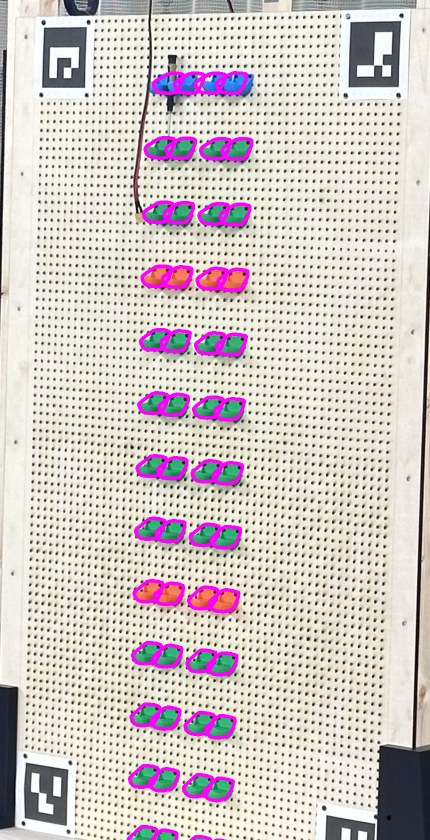
\includegraphics[width=\textwidth]{img/real_holds.jpg}
\caption{Les 52 prises trouvées (contours magenta).}
\end{subfigure}\hspace{0.05\textwidth}%
\begin{subfigure}[b]{0.36\textwidth}
\centering
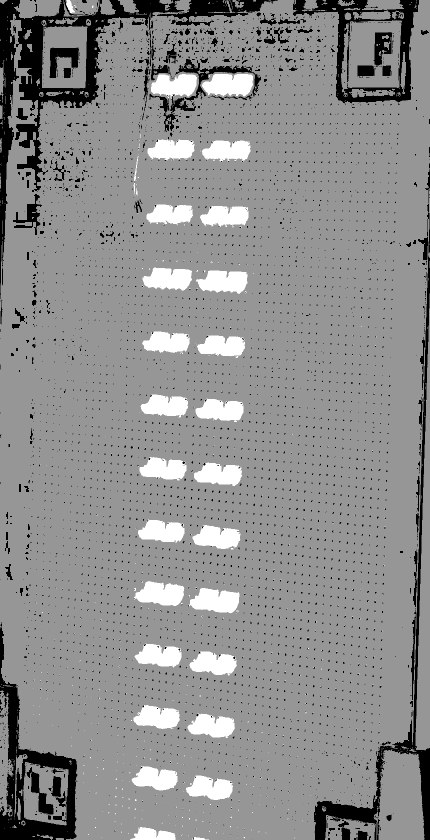
\includegraphics[width=\textwidth]{img/real_classes.jpg}
\caption{Les classes : blanc = prise, gris = mur, noir = inconnu.}
\end{subfigure}
\caption{La détection des prises sur la photo du vrai mur (recadrée sur le mur).}
\label{fig:reel}
\end{figure}

\begin{itemize}
  \item \textbf{52 prises trouvées} : 13 rangées de 4, aux rangées 2, 9, 16\ldots{} 86 (une rangée tous les 105~mm) et aux
        colonnes \textbf{18, 21, 26 et 29} : l'échelle du mur N2, prises de mains à l'extérieur, de pieds à l'intérieur.
  \item \textbf{Les couleurs sont justes} : bleu pour la rangée du haut (86), orange pour les rangées 30 et 65, vert pour
        les autres --- exactement la photo.
  \item \textbf{À vérifier} : la rangée bleue du haut sort aux colonnes 19, 22, 25 et 28, décalée d'une colonne vers
        l'intérieur, alors qu'elle semble alignée sur les autres. L'accroche de la corde passe devant, et la focale du
        téléphone n'est qu'estimée.
  \item \textbf{Ce que l'essai a corrigé} : d'abord 42 prises, car le contreplaqué réel, presque blanc, était classé
        « inconnu » (seuil de gris abaissé de 40 à 10) ; puis 28, une par paire, au milieu des paires collées (échange
        « une prise $\to$ deux ») ; enfin 52.
\end{itemize}

% =========================================================================================================
\section{Pour le vrai robot}

\begin{enumerate}
  \item \textbf{Brancher les deux caméras} en USB sur l'ordinateur de l'équipe. Les organisateurs les placent ; il ne
        faut pas les déplacer, et rien n'est à mesurer.
  \item \textbf{Trouver leurs numéros} : lancer \code{live.py 0 1}, puis 1 2, 2 3\ldots{} jusqu'à voir les deux images
        couleur. \textbf{Seule l'image couleur (RGB) est autorisée} par le règlement.
  \item \textbf{Calibrer les intrinsèques} de chaque caméra (une fois), \textbf{en 1920~×~1080} : soit lire les valeurs
        d'usine de la RealSense (\code{rs2_intrinsics}), soit faire une calibration OpenCV avec un damier. Les écrire
        dans un fichier \code{cams.json} :
\begin{lstlisting}
{"cameras": [
  {"name": "cam_left",  "width": 1920, "height": 1080,
   "fx": 1365.4, "fy": 1364.8, "cx": 961.9, "cy": 543.0, "dist": [0, 0, 0, 0, 0]},
  {"name": "cam_right", "width": 1920, "height": 1080,
   "fx": 1368.7, "fy": 1367.9, "cx": 956.7, "cy": 539.1, "dist": [0, 0, 0, 0, 0]}]}
\end{lstlisting}
        (valeurs d'exemple). La clé \code{dist} n'est lue que par \code{live.py} : garder un fichier séparé pour l'éditeur
        de caméras du simulateur.
  \item \textbf{Imprimer la fiche du marqueur ID~5} à 100~\%, vérifier la règle de 100~mm et le code de 42~mm, découper le
        contour, coller l'autocollant à plat sur le dos, l'encoche en butée contre le pied de la poignée.
  \item \textbf{Vérifier la calibration} avec l'éditeur de caméras du simulateur : y charger une photo de la vraie
        caméra et les paramètres trouvés ; le mur dessiné par-dessus doit tomber exactement sur le vrai mur.
\begin{lstlisting}[style=sh]
uv run climbing-sim-cameras
\end{lstlisting}
  \item \textbf{À chaque essai}, \emph{avant} de mettre le robot sur le mur : appuyer sur \textbf{c} (caméras et
        prises), vérifier que chaque caméra voit \code{[1, 2, 3, 4]} avec une reprojection inférieure à 1~pixel, et
        avec \textbf{h} que la liste des prises est complète et sans fausse prise.
  \item \textbf{Les couleurs} : si une prise réelle est mal vue (couleur pâle, éclairage), ajuster les seuils
        \code{HOLD_SAT_MIN} et \code{GREY_SAT_MAX} en tête de la partie « holds » de \code{perception.py}.
\end{enumerate}

\begin{attention}[Ce qui n'a pas pu être testé]
La lecture de vraies caméras USB n'a pas été testée : pas de matériel, et la webcam de l'ordinateur n'a pas été
ouverte. Le premier essai sur place doit vérifier le numéro des caméras, la résolution (1920~×~1080) et que l'image
reçue est bien l'image couleur. La détection des prises n'a été essayée que sur une photo de téléphone.
\end{attention}

% =========================================================================================================
\section{Limites et prochaines étapes}
\label{sec:suite}

\subsection{Limites connues}

\begin{itemize}
  \item \textbf{L'IMU du vrai robot n'est pas encore reliée à \code{live.py}} : sur le vrai robot, le suivi utilise
        le marqueur seul (environ 2,5~mm en moyenne dans le simulateur, contre 1~mm avec l'IMU). Il faudra transmettre
        la gravité mesurée par le robot (\code{obs["gravity"]}) à \code{tracker.update()}.
  \item \textbf{Occultation} : si un bras passe devant le marqueur dans une caméra, \code{update()} renvoie
        \code{None} (une caméra ne suffit pas). Le programme de grimpe doit le prévoir (garder la dernière pose connue,
        ou utiliser les angles des moteurs).
  \item \textbf{Prises cachées} : une prise que le robot cache aux deux caméras n'est pas vue tant qu'il est devant ;
        d'où l'intérêt de chercher les prises avant de mettre le robot sur le mur, puis de cumuler.
  \item \textbf{Simulateur idéal} : images sans flou, sans bruit, sans distorsion, éclairage parfait. Les vraies images
        seront moins nettes : la précision réelle sera moins bonne que ces chiffres.
  \item \textbf{Pénalité} : le mode avec marqueurs multiplie le temps par 1,25.
\end{itemize}

\subsection{Prochaines étapes}

\begin{enumerate}
  \item \textbf{Écrire le programme de grimpe} : bouger un membre à la fois en gardant les trois autres accrochés, avec
        la cinématique inverse du simulateur, en s'appuyant sur la position du tronc et des prises données par le
        \code{Tracker}.
  \item \textbf{Relier l'IMU du vrai robot} à \code{live.py}.
  \item \textbf{Essayer avec les vraies caméras} et le vrai mur, et ajuster les seuils de couleur si besoin.
\end{enumerate}

% =========================================================================================================
\appendix
\section{Aide-mémoire des commandes}

\begin{lstlisting}[style=sh]
cd ~/Desktop/Hackathon/simulator          # toujours depuis ce dossier

# demonstration (mur N1, N2 ou N3), avec une fenetre ; la video
uv run --with opencv-contrib-python python ../perception/demo.py N2 --show
open ../perception/out/demo.mp4
# cameras au hasard, autre resolution
uv run --with opencv-contrib-python python ../perception/demo.py N2 --shuffle 3
uv run --with opencv-contrib-python python ../perception/demo.py N2 --res 1280x720

# les prises trouvees, dans l'editeur de mur
uv run climbing-sim-wall-editor ../perception/out/holds.json

# le jour J : cameras USB (gauche puis droite), avec ou sans calibration
uv run --with opencv-contrib-python python ../perception/live.py 0 1
uv run --with opencv-contrib-python python ../perception/live.py 0 1 --cameras cams.json

# sur des images, sans fenetre (ici les images brutes laissees par la demo)
uv run --with opencv-contrib-python python ../perception/live.py \
    ../perception/out/cam_left_raw.png ../perception/out/cam_right_raw.png --once

# verifier la calibration des cameras sur une photo (outil du simulateur)
uv run climbing-sim-cameras

# regenerer les images de ce document, puis le compiler
uv run --with opencv-contrib-python python ../perception/doc/make_figures.py
cd ../perception/doc && latexmk -xelatex perception_aruco.tex
\end{lstlisting}

\section{Référence des fonctions}

\begin{center}
\renewcommand{\arraystretch}{1.2}
\begin{tabularx}{\textwidth}{>{\raggedright}p{5.4cm} X}
\toprule
Fonction & Rôle \\
\midrule
\multicolumn{2}{l}{\textbf{\code{perception.py}}} \\
\code{detect(image)} & marqueurs d'une image RGB : \code{{ID: 4 coins en pixels}} \\
\code{wall_marker_corners(id)} & les 4 coins du code d'un marqueur du mur, en 3D (repère mur) \\
\code{camera_pose(markers, K, dist)} & pose d'une caméra à partir des marqueurs 1--4 : \code{(rvec, tvec, rms)} \\
\code{marker_pose(views, size)} & pose d'un marqueur dans le repère du mur (triangulation, ou PnP avec une caméra) \\
\code{robot_pose(views, size, R, p)} & pose du tronc dans le repère du mur \\
\code{level_with_gravity(pose, g, p)} & la même, inclinaison corrigée par la gravité de l'IMU \\
\code{to_world(R, p)} & repère du mur $\to$ repère du simulateur \\
\code{pixel_classes(image)} & classe de chaque pixel : prise, mur ou inconnu \\
\code{hold_candidates()}, \code{hold_points()} & les places possibles des prises ; 200 points de la prise \\
\code{hold_pixels()}, \code{hold_votes()} & projection des places dans une caméra ; votes d'une image \\
\code{select_holds(hit, known, seen)} & les prises, d'après les votes (seuils, chevauchements, paires) \\
\code{FoundHold} & une prise trouvée : \code{hold} (\code{col}, \code{row}, \code{socket}), \code{socket_wall}, \code{color}, \code{score}, \code{seen} \\
\code{annotate(image, tracker, nom, pose, holds)} & image annotée (marqueurs, prises, repère du tronc) \\
\code{Tracker} & le tout : \code{calibrate()}, \code{find_holds()}, \code{reset_holds()}, \code{update(images, gravity)} ;
  \code{min_views} (2), \code{seen_by} \\
\midrule
\multicolumn{2}{l}{\textbf{\code{robot_marker.py}}} \\
\code{CODE}, \code{R_TRUNK_MARKER}, \code{P_TRUNK_MARKER} & le marqueur ID~5 de la fiche : 42~mm, axes, centre $(-33; 0; 54{,}75)$~mm \\
\code{MarkedSim(...)} & \code{ClimbingSim} avec l'autocollant sur le dos \\
\code{add_robot_marker(spec)}, \code{sticker_image()} & ajoute l'autocollant à une scène ; son image \\
\bottomrule
\end{tabularx}
\end{center}

\section{Petit glossaire}

\begin{description}[style=nextline, leftmargin=1.2em, font=\normalfont\bfseries]
  \item[Pose] position et orientation d'un objet (6 nombres : 3 pour la position, 3 pour la rotation).
  \item[Intrinsèques] paramètres propres à une caméra (focale, centre de l'image, distorsion) ; ne changent pas
        quand on la déplace.
  \item[Extrinsèques] pose de la caméra par rapport au monde (ici, au mur) ; changent dès qu'on la bouge.
  \item[PnP] (\emph{Perspective-n-Point}) retrouver la pose d'une caméra à partir de points 3D connus et de
        leurs pixels.
  \item[Erreur de reprojection] écart, en pixels, entre les points détectés et ceux recalculés avec la pose
        trouvée ; mesure la qualité d'une calibration.
  \item[Triangulation] retrouver un point 3D comme l'intersection des rayons de deux caméras.
  \item[Kabsch] méthode qui trouve la rotation et la translation superposant au mieux deux nuages de points.
  \item[IPPE] méthode de PnP exacte pour des points dans un même plan (\code{SOLVEPNP_IPPE}), et sa variante pour un
        marqueur carré seul (\code{SOLVEPNP_IPPE_SQUARE}).
  \item[IMU] centrale inertielle du robot : gyroscope et accéléromètre ; donne la direction de la gravité, donc son
        inclinaison, mais pas son cap.
  \item[Saturation] vivacité d'une couleur (0 : gris, 255 : couleur pure) ; elle sépare les prises du bois pâle.
  \item[Coupelle (socket)] le creux de la prise où se pose la boule au bout de chaque membre du robot.
\end{description}

\end{document}
